\newcommand{\mgn}{\mathcal M_{g,n}}
\newcommand{\mgnb}{\overline{\mathcal M_{g,n}}}
\newcommand{\mgb}[1]{\overline{\mathcal M_{g,#1}}}

\documentclass[11pt]{article}           % 11pt article
\makeatletter                   % Make '@' accessible.
\pagestyle{myheadings}              % We do our own page headers.
\oddsidemargin=0in              % Left margin minus 1 inch.
\evensidemargin=0in             % Same for even-numbered pages.
\textwidth=6.5in                % Text width (8.5in - margins).
\topmargin=0in                  % Top margin minus 1 inch.
\headsep=0.2in                  % Distance from header to body.
\textheight=8in                 % Body height (incl. footnotes)
\skip\footins=4ex               % Space above first footnote.
\hbadness=10000                 % No "underfull hbox" messages.
\makeatother                    % Make '@' special again.

%==============================================================================
% Packages used (packages add more commands)
%==============================================================================

\usepackage{amsmath}                % give more fonts and symbols
\usepackage{amsfonts}               % want AMS fonts
\usepackage{amssymb}
\usepackage{amsthm}
\usepackage{mathrsfs}
\usepackage{tikz-cd}
\usepackage[shortlabels]{enumitem}
\usepackage{relsize}
\usepackage{hyperref}
\usepackage{biblatex}
\addbibresource{sources.bib}

\makeatletter
\newcommand*{\relrelbarsep}{.386ex}
\newcommand*{\relrelbar}{%
  \mathrel{%
    \mathpalette\@relrelbar\relrelbarsep
  }%
}
\newcommand*{\@relrelbar}[2]{%
  \raise#2\hbox to 0pt{$\m@th#1\relbar$\hss}%
  \lower#2\hbox{$\m@th#1\relbar$}%
}
\providecommand*{\rightrightarrowsfill@}{%
  \arrowfill@\relrelbar\relrelbar\rightrightarrows
}
\providecommand*{\leftleftarrowsfill@}{%
  \arrowfill@\leftleftarrows\relrelbar\relrelbar
}
\providecommand*{\xrightrightarrows}[2][]{%
  \ext@arrow 0359\rightrightarrowsfill@{#1}{#2}%
}
\providecommand*{\xleftleftarrows}[2][]{%
  \ext@arrow 3095\leftleftarrowsfill@{#1}{#2}%
}
\makeatother

%==============================================================================
% Macros (make your own commands)
%==============================================================================

% For problem and part headers
\newcounter{problemcounter}
\newcounter{subproblemcounter}
\newcommand{\problem}{
    \addtocounter{problemcounter}{1}
    \bigskip
    \noindent {\Large Problem \hwnumber .\theproblemcounter}
    \smallskip
    \setcounter{subproblemcounter}{0}
}
\newcommand{\subproblem}{
    \addtocounter{subproblemcounter}{1}
    \smallskip
    \noindent {\bf \alph{subproblemcounter})} 
}

% Nice things
\newcommand{\set}[1]{\{#1\}}            % Set (as in \set{1,2,3})
\newcommand{\setof}[2]{\{\,{#1}|~{#2}\,\}}  % Set (as in \setof{x}{x > 0})

% Some letter symbols
\newcommand{\N}{\ensuremath{\mathbb{N}}}
\newcommand{\Z}{\ensuremath{\mathbb{Z}}}
\newcommand{\R}{\ensuremath{\mathbb{R}}}
\newcommand{\hTop}{\textbf{hTop}}
\newtheorem*{Proposition}{Proposition}
\newtheorem*{Corollary}{Corollary}
\newcommand{\Tor}{\text{Tor}}
\newcommand{\Ext}{\text{Ext}}
\newcommand{\Q}{\mathbb{Q}}
\newcommand{\F}{\mathbb{F}}
\newcommand{\C}{\mathbb{C}}
\newcommand{\CP}{\mathbb{CP}}
\newcommand{\RP}{\mathbb{RP}}
\newcommand{\Spec}{\text{Spec}}
\newcommand{\Aut}{\text{Aut}}
\newcommand{\Proj}{\text{Proj}}
\newcommand{\Mor}{\text{Mor}}
\newcommand{\codim}{\text{codim}}
\newcommand{\exer}[1]{{\bf Exercise #1} \\}
\newcommand{\Hom}{\text{Hom}}
\newcommand{\coker}{\text{coker}}
\newcommand*\simplex{\includegraphics[scale=0.017]{simplex.png}}
\newcommand{\Sch}{\textbf{Sch}}
\newcommand{\Set}{\textbf{Set}}
\newcommand{\Hb}{\overline{\mathcal H}}
\renewcommand{\a}{\mathfrak a}
\renewcommand{\b}{\mathfrak b}
\renewcommand{\P}{\mathbb P}
\theoremstyle{definition}
\newtheorem*{thm}{Theorem}
\newtheorem*{prob}{Problem}
\newtheorem*{dfn}{Definition}
\newtheorem*{claim}{Claim}
\theoremstyle{definition}
\newtheorem*{lem}{Lemma}
\newtheorem*{ex}{Exercise}
\newtheorem*{eg}{Example}
\newtheorem*{note}{Note}

\usetikzlibrary{matrix,positioning,quotes}

%==============================================================================
% YOUR DOCUMENT (start here)
%==============================================================================

\definecolor{myblue}{RGB}{100,180,255}
\definecolor{mygreen}{RGB}{80,160,80}
\definecolor{myred}{RGB}{200,120,100}


\begin{document}

\title{Reverse Hurwitz counts of genus $1$ curves}

\author{Michael Mueller}

\maketitle


\tableofcontents

\section{Introduction}

\subsection{Moduli spaces of curves (basic intro)}

Include stable graphs

\subsection{Moduli spaces of maps}

Include maps of stable graphs

\subsection{Hurwitz theory}

Include marked and unmarked

\subsection{Comparison with other invariants}

Comparison with generalized Tevelev degrees

Admissible covers

\section{Problem statement and general approaches}

\subsection{Definitions}
Fix a positive integer $d$, a nonnegative integer $g$, ordered partitions $\sigma_1,\dots,\sigma_n$ of $d$, and subpartitions $\nu_1,\dots,\nu_n$ (i.e., $\nu_i$ is a subset of $\sigma_i$).

Let $\Hb_{g,\sigma}$ be the moduli space of degree $d$ admissible covers $C\to X$
where $C$ is a genus $g$ prestable curve, $X$ is a genus $0$ prestable curve, we have marked points $q_1,\dots,q_n\in X$, the ramification profile over $q_i$ is $\sigma_i$, and the map is \'etale away from $q_1,\dots,q_n$. This situation is described in Figure \ref{fig:hurwitz}.

\begin{figure}[h]
  \caption{Depiction of a Hurwitz cover with notation used in this thesis}
  \centering
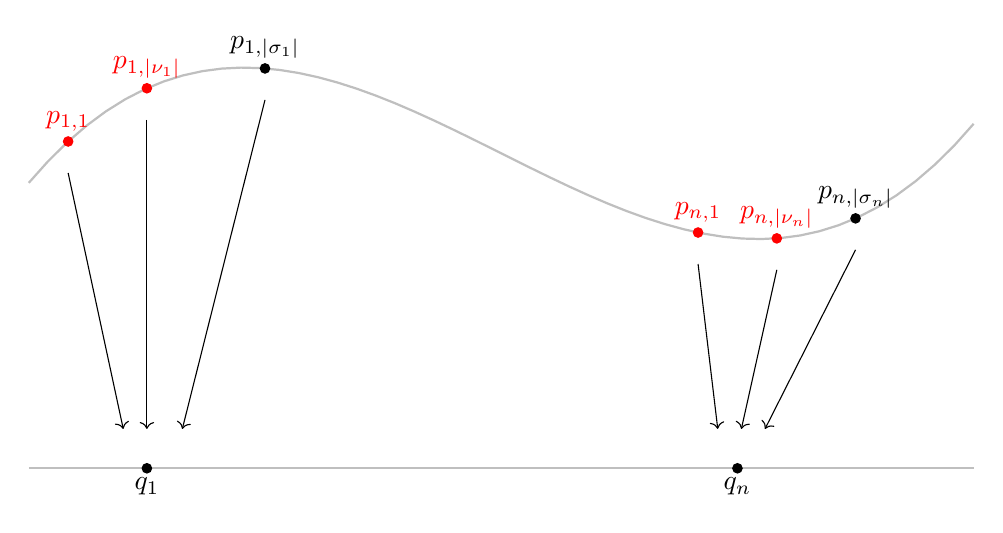
\begin{tikzpicture}
  \draw[domain=-6:6,samples=50,color=gray!50,thick] plot (\x, \x^3/64 - \x/2);
  \foreach \x/\p/\c in {-5.5/$p_{1,1}$/red, -4.5/$p_{1,|\nu_1|}$/red, -3/$p_{1,|\sigma_1|}$/black}
  {
    \filldraw[\c] (\x,\x^3/64 - \x/2) circle (0.6mm) node[above] {\p};
    \draw[->] (\x,\x^3/64 - \x/2 - .4) -- (-3.15+.3*\x, -3.5);
    }
  \foreach \x/\p/\c in {2.5/$p_{n,1}$/red, 3.5/$p_{n,|\nu_n|}$/red, 4.5/$p_{n,|\sigma_n|}$/black}
  {
    \filldraw[\c] (\x,\x^3/64 - \x/2) circle (0.6mm) node[above] {\p};
    \draw[->] (\x,\x^3/64 - \x/2 - .4) -- (2+.3*\x, -3.5);
    }

    \draw[domain=-6:6,samples=50,color=gray!50,thick] plot (\x, -4);
  \foreach \x/\q in {-4.5/$q_1$, 3/$q_n$}
    \filldraw[black] (\x,-4) circle (0.6mm) node[below] {\q};
\end{tikzpicture}

\label{fig:hurwitz}
\end{figure}

%TODO: something other than color, for accessibility?


Let $m=\sum|\nu_i|$ and $N=\sum|\sigma_i|$.
We have natural maps:

\begin{tikzcd}
\overline{\mathcal M}_{0,n} & \ar[l,""] \Hb_{g,\sigma} \ar[r,""] \ar[rr,out=-30,in=210,"\pi_{\nu}"] & \overline{\mathcal M}_{g,N} \ar[r,""] & \overline{\mathcal M}_{g,m}
\end{tikzcd}

Here $\pi_{\nu}$ remembers the source curve and red points, i.e.\ the points corresponding to $\nu$.
By Hurwitz theory, we know that the first map is finite, and so $\dim(\Hb_{\sigma,\mu})=n-3$. The second map $\pi_{\nu}$ is finite when
\begin{align*}
  \label{eqn:dimension}
3g-3+m=n-3\iff 3g+m=n
\end{align*}
and in this case, we define
\[
W_{g,\sigma,\nu}=\deg(\pi_{\nu})
\]
where this is an orbifold degree.
In order to account for relabeling of marked points (any of the points $q_n$ with identical data, as well as any of the unmarked points in fibers with
identical data), we define
\[
N_{g,\sigma,\nu}=\frac{W_{g,\sigma,\nu}}{|\Aut(\{(\sigma_i,\nu_i):1\leq i\leq n\})|\cdot \prod_i|\Aut(\sigma_i-\nu_i)|}
\]
In many cases studied in this thesis, we will specialize to the case where $g=1$,
$\sigma_1=\nu_1=\mu$, and $\nu_3=\nu_4=\dots=\emptyset$. We will write
\[
W_{\sigma_1,\dots,\sigma_n}^{\lambda}(\mu)=W_{1,(\mu,\sigma_1,\dots,\sigma_n),(\lambda,\emptyset,\dots,\emptyset)}
\]
for the relevant labeled invariant, and
\[
N_{\sigma_1,\dots,\sigma_n}^{\lambda}(\mu)=N_{1,(\mu,\sigma_1,\dots,\sigma_n),(\lambda,\emptyset,\dots,\emptyset)}
\]
for the unlabeled invariant that will be of most interest to us. In particular we will write
\[
N_{\sigma_1,\dots,\sigma_n}(\mu)=N_{\sigma_1,\dots,\sigma_n}^{\emptyset}(\mu)=\frac{W_{\sigma_1,\dots,\sigma_n}^{\emptyset}(\mu)}{|\Aut(\sigma_2,\dots,\sigma_n)|\cdot\prod_{i=2}^n|\Aut(\sigma_i)|}
\]
If $\mu,\sigma_1,\dots,\sigma_n$ do not have ramification sufficient to satisfy Riemann-Hurwitz,
we let \[N_{\sigma_1,\dots,\sigma_n}(\mu) = N_{\sigma_1,\dots,\sigma_n,(2,1^{d-2}),\dots}(\mu).\]
The primary task of this thesis is to understand the invariants $N_{\sigma_1,\dots,\sigma_n}(\mu)$
in some significant special cases.

\begin{eg}
  Consider the case where $d=2$, $n=1$ and $\mu=\sigma_1=\sigma_2=\sigma_3=(2)$.
  We know that there is a unique map $(E,p)\to (\mathbb P^1,0)$ of the specified form
  up to automorphisms of $\P^1$, and it factors through the antipodal automorphism of $E$,
  so
  \[
  N(2)=N_{(2),(2),(2)}(2)=1. %TODO: why is it not 1/2?
  \]
\end{eg}

\begin{eg}
  Consider the case where $g=0$, $\sigma=(\sigma_1,\sigma_2,\sigma_3)$ and $m=3$. In this case
  \[
  W_{0,\sigma,\nu}=\overline H(\sigma_1,\sigma_2,\sigma_3)
  \]
  where $\overline H$ is a marked Hurwitz number.
  \end{eg}

\subsection{Notation and conventions}

\subsection{Geometric interpretation and examples}
We can describe $N_{\mu,\sigma_2,\dots,\sigma_n}$ geometrically as follows.

Let $d>2$. Up to automorphisms of $\P^1$, a degree $d$ map $f:E\to\P^1$ corresponds to a degree $d$ line bundle $\mathcal L$ and a basepoint-free two-dimensional subspace $V\subset H^0(\mathcal L)$. By Riemann-Roch, $\mathcal L$ gives an embedding $E\hookrightarrow\P(H^0(\mathcal L))\cong\P^{d-1}$, and a basepoint-free two-dimensional subspace $V\subset H^0(\mathcal L)$ corresponds to a well-defined composition
\[
E\hookrightarrow \P(H^0(\mathcal L))=\P(V\oplus V^{\perp})\dashrightarrow\P(V)\cong\P^1
\]
For the composition to be well-defined, $E$ should not intersect $\P(V^{\perp})$, a codimension 2 subspace of $\P(H^0(\mathcal L))$. Each fiber of the rational map
$\P(V\oplus V^{\perp})\dashrightarrow\P(V)$ is a hyperplane containing $\P(V^{\perp})$, and so the fibers of the map $E\to\P^1$ correspond to intersections $H\cap E$ where $H$ is some hyperplane containing $\P(V^{\perp})$. Thus, $N_{\mu,\sigma_2\dots,\sigma_n}$ can be determined by embedding $E$ in $\P^{d-1}$ via $\mathcal L=\mathcal O(\mu_{1}p_1+\dots+\mu_{|\mu|}p_{|\mu|})$ and counting the number of codimension 2 subspaces $\P(V^{\perp})\subset \P^{d-1}$ such that (a) $\P(V^{\perp})\cap E=\emptyset$, (b) $\P(V^{\perp})\subset H_0$ where $H_0\cap E=\mu_{1}p_1+\dots+\mu_{|\mu|}p_{|\mu|}$, (c) $\P(V^{\perp})\subset H_i$ where $H_i\cap E$ has shape $\sigma_i$, for $i=2,\dots,n$.

Note that if $\P(V^{\perp})$ is such a codimension 2 subspace corresponding to a map $f$, then $-\P(V^{\perp})$ (applying the involution on $E$, which extends to an automorphism of $\P(H^0(\mathcal L))$) is as well and corresponds to $x\mapsto f(-x)$.

\begin{eg}
  Let's compute $N_{(3),(3)}$. Embedding $E\hookrightarrow\P^2$ via $\mathcal L=\mathcal O(3p)$, we want to count the points $q\notin E$ such that
  $q\in\ell_0$ (the line at infinity) and $q\in\ell_1$, where $\ell_1\cap E=3r$ for some $r\neq p$ (we don't need to worry about the simple ramification, which
  is guaranteed). Since $q=\ell_0\cap\ell_1$ we just need to count lines $\ell_1$ with $\ell_1\cap E=3r$ for $r\neq p$; these are flex lines corresponding to nontrivial 3-torsion points, of which there are $3^2-1=8$. Therefore,
  \[
  N_{(3),(3)}=8.
  \]
\end{eg}
\begin{eg}
  Let's compute $N_{(2,1),(3)}$. If $\mathcal O(2p_1+p_2)=\mathcal O(3p_{\infty})$, then we can embed $E$ in $\P^2$ with $p_{\infty}$ as the point at infinity
  and let $\ell_0$ be a line such that $\ell_0\cap E=2p_1+p_2$. We want to count points $q\notin E$ with $q\in \ell_0$ and $q\in \ell_1$, where $\ell_1$ is a flex line. This again amounts to counting flex lines, so $N_{(2,1),(3)}=3^2=9$.

  For similar reasons, $N_{(1,1,1),(3)}=9$.
\end{eg}

Another way to count $N_{\mu_0,\dots,\mu_{n+2}}$: note that $\{H:\P(V^{\perp})\subset H\}$ is a line in $\P(H^0(\mathcal L))^*$.
Let $X_{\mu}=\{H\in\P(H^0(\mathcal L))^*:H\cap E\text{ has shape }\mu\}$.
Counting the number of possibilities $\P(V^{\perp})$ amounts to counting lines $\ell\subset\P(H^0(\mathcal L))^*$ such that $H_0\in\ell$, $H_1,\dots,H_{n+2}\in\ell$ for distinct points $H_i\in X_{\mu_i}$, and $\P(V^{\perp})\cap E=H_0\cap H_1\cap E=\emptyset$.
Letting $\pi:\P^{d-1}\dashrightarrow \{\text{lines in $\P^{d-1}$ through $H_0$}\}=\P^{d-2}$ send $x$ to the line through $x$ and $H_0$, the idea is to count points in $\P^{d-2}$ whose fiber contains distinct points $H_i\in X_{\mu_i}$. (TODO: ensure $\ell$ isn't contained in $\{H:p\in H\}$, a plane in $(\P^3)^*$)

Now we move on to $d=4$, and embed $E$ in $\P^3$ via
$\mathcal L=\mathcal O(4p)$. We have a stratification of $(\P^3)^*$:

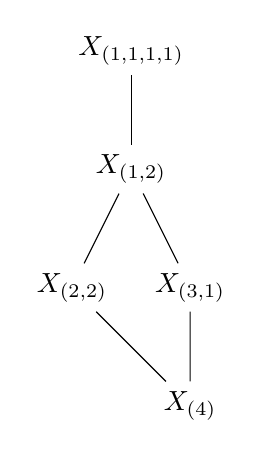
\begin{tikzpicture}
  \node {$X_{(1,1,1,1)}$}
  child {node {$X_{(1,2)}$}
    child {node[name=A] {$X_{(2,2)}$}}
    child {node {$X_{(3,1)}$}
      child {node[name=B] {$X_{(4)}$}}}};
  \draw (A) edge (B);
\end{tikzpicture}

First, note that \[X_{(2,2)}\cong\{(x,y)\in E^2:2x+2y=0\}=\{(x,y)\in E^2:x+y\text{ is 2-torsion}\}\]
so $X_{(2,2)}$ is a disjoint union of four curves each corresponding to a 2-torsion point $t_i$:
\[
C_i=\text{image}(f_i:E\hookrightarrow(\P^3)^*),\ f_i(x)=H\text{ where }H\cap E=2x+2(t_i-x)
\]
Note that $f_i$ is 2-to-1 ($x$ and $t_i-x$ are in the same fiber), so $C_i\cong E/S_2\cong\P^1$.

See ``Documents/four\_curves\_linear.m2'' for the computation in M2 to compute $X_{(2,2)}$; it turns out that each $C_i$ is a plane conic. By counting points of
intersection of the images of $C_i$ under $\pi:(\P^3)^*\dashrightarrow\P^2$, we find that
\[
N_{(4),(2,2),(2,2)}=3
\]
as expected from the Hurwitz calculation. By changing $\pi$ (and therefore $H_0$), we can also find
\[
N_{(3,1),(2,2),(2,2)}=N_{(2,2),(2,2),(2,2)}=6,\]\[ N_{(2,1,1),(2,2),(2,2)}=12,\ N_{(1,1,1,1),(2,2),(2,2)}=24
\]

Next we consider $X_{(3,1)}$ (calculated in ``osculating.m2''). There is a map $g:E\to(\P^3)^*$ sending $q\mapsto H$ where $H$ is the {\it osculating plane} to $E$ at $q$, i.e.\ $H$ intersects $E$ at
$q$ with multiplicity at least 3. This $H$ can be defined as the limit of planes containing $q,r,s\in E$ as $r,s\to q$, or equivalently as the limit of planes containing
$T_qE$ and $r$ as $r\to q$. (TODO: re-work the osculating plane stuff using that it's generated by $v(0),v'(0),v''(0)$.)

Let $E=\{F=G=0\}\subset\P^3$. We know that \[T_qE=\{x:\nabla_qF\cdot x=\nabla_qG\cdot x=0\}\]
A plane containing this tangent line must be of the form \[H=\{x:(a\nabla_qF+b\nabla_qG)\cdot x=0\}\]
for some $a,b$. If $r\in H$, then
\[
a\nabla_qF\cdot r+b\nabla_qG\cdot r=0\implies [a:b]=[\nabla_qG\cdot r:-\nabla_qF\cdot r]
\]
This equation fails when $r=q$ (since $\nabla_qF\cdot q=\nabla_qG\cdot q=0$). Letting $[u:v]$ be the limit of $[\nabla_qG\cdot r:\nabla_qF\cdot r]$
as $r\to q$, we'll have
\[
H=\left\{\left(u\frac{\partial F}{\partial x}\bigg|_q-v\frac{\partial G}{\partial x}\bigg|_q\right)x+
\left(u\frac{\partial F}{\partial y}\bigg|_q-v\frac{\partial G}{\partial y}\bigg|_q\right)y+
\left(u\frac{\partial F}{\partial z}\bigg|_q-v\frac{\partial G}{\partial z}\bigg|_q\right)z+
\left(u\frac{\partial F}{\partial w}\bigg|_q-v\frac{\partial G}{\partial w}\bigg|_q\right)w=0\right\}
\]
It remains to find $u$ and $v$. Suppose we have a (non-algebraic) parametrization of $E$ labeled $v(t)$, with $v(0)=q$. Using L'Hopital, our goal
is to find
\[
\lim_{t\to 0}[\nabla_qG\cdot v(t):\nabla_qF\cdot v(t)]=\lim_{t\to 0}[\nabla_qG\cdot v'(t):\nabla_qF\cdot v'(t)]=\lim_{t\to 0}[\nabla_qG\cdot v''(t):\nabla_qF\cdot v''(t)]=[\nabla_qG\cdot v''(0):\nabla_qF\cdot v''(0)]
\]


We know
$F(v(t))=0$ and $G(v(t))=0$ so
\[
\nabla _{v(t)}F\cdot v'(t)=\nabla _{v(t)}G\cdot v'(t)=0
\]
Taking derivatives again,
\[
\nabla_{v(t)}F\cdot v''(t)+v'(t)\cdot\left(\frac{\partial^2F}{\partial t_i\partial t_j}\right)\cdot v'(t)=\nabla_{v(t)}G\cdot v''(t)+v'(t)\cdot\left(\frac{\partial^2G}{\partial t_i\partial t_j}\right)\cdot v'(t)=0
\]
It remains to compute $v'(0)\cdot H\cdot v'(0)$ where $H$ is the Hessian of $F$ or $G$.
We know that $v'(0)$ is in the kernel of $\nabla_qF$ and $\nabla_qG$ and any generic element of both kernels will work, so we choose an element of the kernel of
\[
\begin{bmatrix}
  \frac{\partial F}{\partial x}\big|_q & \frac{\partial F}{\partial y}\big|_q & \frac{\partial F}{\partial z}\big|_q & \frac{\partial F}{\partial w}\big|_q \\
  \frac{\partial G}{\partial x}\big|_q & \frac{\partial G}{\partial y}\big|_q & \frac{\partial G}{\partial z}\big|_q & \frac{\partial G}{\partial w}\big|_q \\
  1 & 0 & 0 & 0 \\
  \end{bmatrix}
\]
It turns out $[D_1,-D_2,D_3,-D_4]$ works where $D_i$ is the determinant of the matrix produced by deleting the $i^{\text{th}}$ column, which can be shown by duplicating rows and taking determinants
(which will be 0).

After doing this it turns out that $X_{(1,3)}$ is a degree 12 curve, with singularities (cusps? TODO) at the planes $H$ with $H\cap E=4q$ for some $q$ (corresponding to the 4-torsion points). There are $4^2=16$ of these singularities.

To compute $N_{(4),(3,1),(3,1)}$, we take the image $Y_{(1,3)}$ under projection from $H_0$. It turns out that $Y_{(1,3)}$ is a degree 10
curve with cusps at the images of 4-torsion points (except for the image of $H_0$, which is a smooth point) and $20$ nodes, so
\[
N_{(4),(3,1),(3,1)}=\frac{20}{2}=10
\]
TODO: calculate $N_{(1,1,1,1),(3,1),(3,1)}$ using genus-degree formula; explain why this doesn't work for higher degree

\section{Admissible covers}

In this section we explain a known method in the literature that we will use
to recursively compute $W_{g,\sigma,\nu}$. This is a method used in \cite{Generalized} to prove Proposition 6, and reliant on a result from \cite{Lian}. We begin by motivating the method, and then illustrate the use of the method as adapted to the specific context of this thesis.

Recall that $W_{g,\sigma,\nu}$ is the degree of the map $\pi_{\nu}:\Hb_{g,\sigma}\to\overline{\mathcal M_{g,m}}$
where $\sum|\nu_i|=m$; our enumerative interpretation is that, for a fixed general $m$-pointed genus $g$ curve $(C,p_1,\dots,p_m)$, $W_{g,\sigma,\nu}$ counts the number of Hurwitz covers of the correct form with source $(C,p_1,\dots,p_m)$. One can hope (and we will see) that the same is roughly true for
a specific $m$-pointed genus $g$ {\it stable} curve lying in a suitable boundary divisor of $\overline{\mathcal M_{g,m}}$.

We first begin with a rough illustration of what we intend to do.

\begin{eg}
  Suppose we are interested in calculating $W_{(3),(2,1),(2,1),(2,1)}(2,1)$, the degree of the map
  \[
  \pi:\Hb_{1,\sigma}\to\overline{\mathcal M_{1,2}}
  \]
  
  Let $A$ be a stable graph consisting of a genus $1$ vertex connected to a genus $0$ vertex, with two legs on the
  genus $0$ vertex:

                  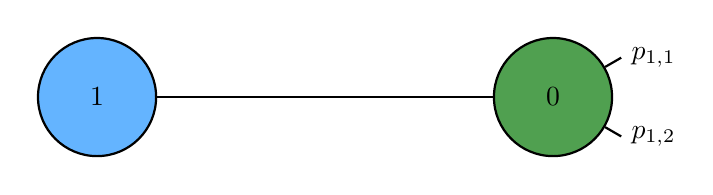
\begin{tikzpicture}[thick,amat/.style={matrix of nodes,nodes in empty cells,
  row sep=3.2em,rounded corners,
  nodes={draw,solid,circle,minimum size=1.5cm}},
  dmat/.style={matrix of nodes,nodes in empty cells,row sep=3.2em,nodes={minimum size=1.5cm},draw=myred},
  fsnode/.style={fill=myblue},
  ssnode/.style={fill=mygreen}]

  \matrix[amat,nodes=fsnode] (mat1) {$1$\\};

 \matrix[amat,right=4cm of mat1,nodes=ssnode] (mat2) {$0$\\};

 \draw  (mat1-1-1) edge (mat2-1-1);
 
  % draw legs for right side
 \draw  (mat2-1-1) -- +(30:1) node[anchor=west] {$p_{1,1}$}
 (mat2-1-1) -- +(330:1) node[anchor=west] {$p_{1,2}$};

              \end{tikzpicture}
  

  Intuitively we want to count covers from a generic stable curve with graph $A$ to a genus $0$
  curve, such that $p_{1,1}$ and $p_{1,2}$ are in the same fiber (with ramification indices $2$ and $1$),
  and there is marked ramification elsewhere with ramification profiles $(3),(2,1),(2,1),(2,1)$.
  Remembering the marked points, the source should be a stable curve in $\overline{\mathcal M_{1,9}}$ with graph $\hat A$, where $\hat A$
  becomes $A$ after applying a forgetful map.

  One possible graph $\hat A_1$, obtained by putting $p_{5,1}$ and $p_{5,2}$ on the genus $0$ component and other
  marked points on the genus $1$ component, is the source of a type of admissible cover in $\Hb_{1,\sigma}$:

                  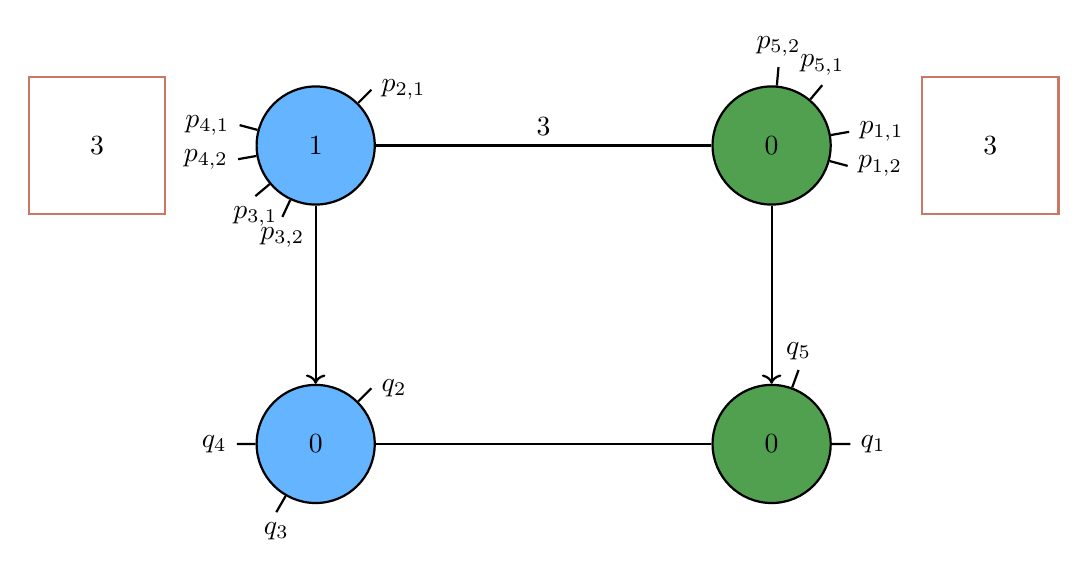
\begin{tikzpicture}[thick,amat/.style={matrix of nodes,nodes in empty cells,
  row sep=3.2em,rounded corners,
  nodes={draw,solid,circle,minimum size=1.5cm}},
  dmat/.style={matrix of nodes,nodes in empty cells,row sep=3.2em,nodes={minimum size=1.5cm},draw=myred},
  fsnode/.style={fill=myblue},
  ssnode/.style={fill=mygreen}]

  \matrix[amat,nodes=fsnode] (mat1) {$1$\\};

    \matrix[dmat,left=1cm of mat1] (degrees1) {$3$\\};


 \matrix[amat,right=4cm of mat1,nodes=ssnode] (mat2) {$0$\\};

 \matrix[dmat,right=1cm of mat2] (degrees2) {$3$\\};

 \draw  (mat1-1-1) edge["$3$"] (mat2-1-1);

  % draw legs for left side
 \draw (mat1-1-1) -- +(45:1) node[anchor=west] {$p_{2,1}$}
 (mat1-1-1) -- +(220:1) node[anchor=north] {$p_{3,1}$}
 (mat1-1-1) -- +(245:1) node[anchor=north] {$p_{3,2}$}
 (mat1-1-1) -- +(165:1) node[anchor=east] {$p_{4,1}$}
 (mat1-1-1) -- +(190:1) node[anchor=east] {$p_{4,2}$};
%  (mat1-1-1) -- +(95:1) node[anchor=south] {$p_{5,1}$}
% (mat1-1-1) -- +(125:1) node[anchor=south] {$p_{5,2}$};

 % draw legs for right side
 \draw  (mat2-1-1) -- +(10:1) node[anchor=west] {$p_{1,1}$}
 (mat2-1-1) -- +(345:1) node[anchor=west] {$p_{1,2}$}
 (mat2-1-1) -- +(50:1) node[anchor=south] {$p_{5,1}$}
 (mat2-1-1) -- +(85:1) node[anchor=south] {$p_{5,2}$};

 \matrix[amat,nodes=fsnode,below=2cm of mat1] (mat3) {$0$\\};

 \matrix[amat,nodes=ssnode,below=2cm of mat2] (mat4) {$0$\\};

  \draw (mat3-1-1) -- +(45:1) node[anchor=west] {$q_2$}
  (mat3-1-1) -- +(180:1) node[anchor=east] {$q_4$}
  (mat3-1-1) -- +(240:1) node[anchor=north] {$q_3$};
   
  \draw  (mat4-1-1) -- +(0:1) node[anchor=west] {$q_1$}
 (mat4-1-1) -- +(70:1) node[anchor=south] {$q_5$};

 \draw  (mat3-1-1) edge[] (mat4-1-1);

 \draw  (mat1-1-1) edge[->] (mat3-1-1);
 \draw  (mat2-1-1) edge[->] (mat4-1-1);

                \end{tikzpicture}

                  Another possible graph $\hat A_2$, obtained by putting $p_{2,1}$ on the genus $0$ component
                  and the other marked points on the genus $1$ component,
                  is the source of another type of admissible cover in $\Hb_{1,\sigma}$:

                                    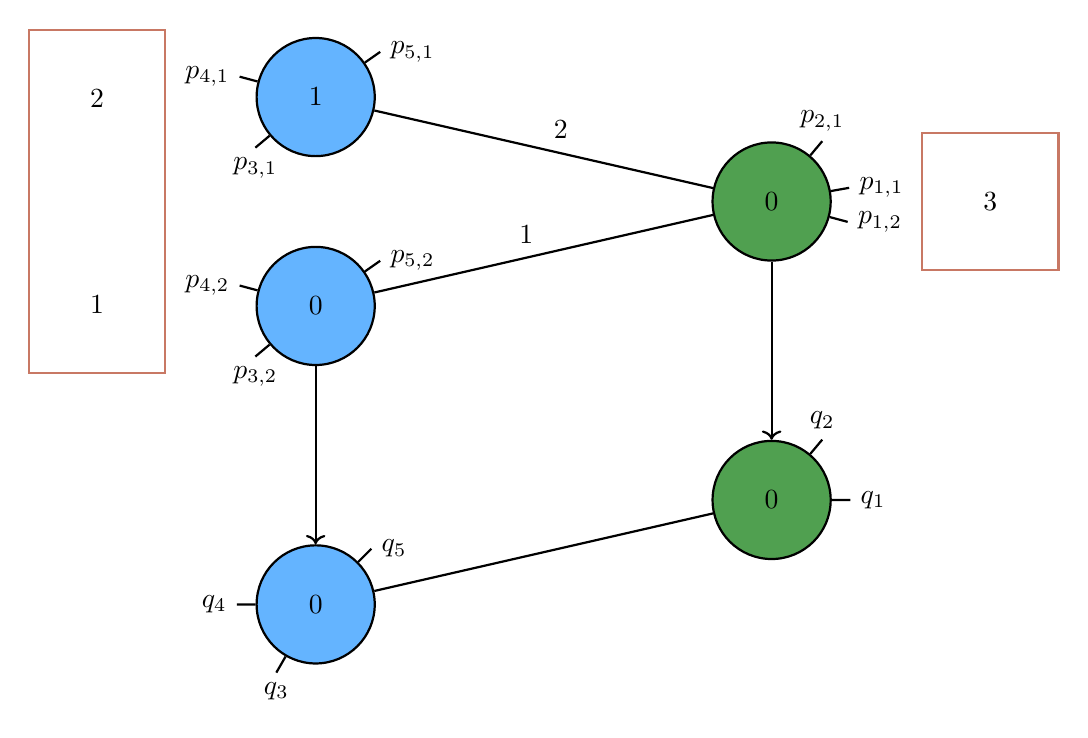
\begin{tikzpicture}[thick,amat/.style={matrix of nodes,nodes in empty cells,
  row sep=3.2em,rounded corners,
  nodes={draw,solid,circle,minimum size=1.5cm}},
  dmat/.style={matrix of nodes,nodes in empty cells,row sep=3.2em,nodes={minimum size=1.5cm},draw=myred},
  fsnode/.style={fill=myblue},
  ssnode/.style={fill=mygreen}]

                                      \matrix[amat,nodes=fsnode] (mat1) {$1$\\
                                      $0$\\};

  \matrix[dmat,left=1cm of mat1] (degrees1) {$2$\\
  $1$\\};


 \matrix[amat,right=4cm of mat1,nodes=ssnode] (mat2) {$0$\\};

 \matrix[dmat,right=1cm of mat2] (degrees2) {$3$\\};

 \draw  (mat1-1-1) edge["$2$"] (mat2-1-1)
 (mat1-2-1) edge["$1$"] (mat2-1-1);

  % draw legs for left side
 \draw (mat1-1-1) -- +(35:1) node[anchor=west] {$p_{5,1}$}
 (mat1-2-1) -- +(35:1) node[anchor=west] {$p_{5,2}$}
 (mat1-1-1) -- +(220:1) node[anchor=north] {$p_{3,1}$}
 (mat1-2-1) -- +(220:1) node[anchor=north] {$p_{3,2}$}
 (mat1-1-1) -- +(165:1) node[anchor=east] {$p_{4,1}$}
 (mat1-2-1) -- +(165:1) node[anchor=east] {$p_{4,2}$};
%  (mat1-1-1) -- +(95:1) node[anchor=south] {$p_{5,1}$}
% (mat1-1-1) -- +(125:1) node[anchor=south] {$p_{5,2}$};

 % draw legs for right side
 \draw  (mat2-1-1) -- +(10:1) node[anchor=west] {$p_{1,1}$}
 (mat2-1-1) -- +(345:1) node[anchor=west] {$p_{1,2}$}
 (mat2-1-1) -- +(50:1) node[anchor=south] {$p_{2,1}$};

 \matrix[amat,nodes=fsnode,below=2cm of mat1] (mat3) {$0$\\};

 \matrix[amat,nodes=ssnode,below=2cm of mat2] (mat4) {$0$\\};

  \draw (mat3-1-1) -- +(45:1) node[anchor=west] {$q_5$}
  (mat3-1-1) -- +(180:1) node[anchor=east] {$q_4$}
  (mat3-1-1) -- +(240:1) node[anchor=north] {$q_3$};
   
  \draw  (mat4-1-1) -- +(0:1) node[anchor=west] {$q_1$}
 (mat4-1-1) -- +(50:1) node[anchor=south] {$q_2$};

 \draw  (mat3-1-1) edge[] (mat4-1-1);

 \draw  (mat1-2-1) edge[->] (mat3-1-1);
 \draw  (mat2-1-1) edge[->] (mat4-1-1);

                \end{tikzpicture}

                                    We hope that $W_{(3),(2,1),(2,1),(2,1)}(2,1)$ can be expressed
                                    as a sum of terms corresponding to these kinds of
                                    admissible covers:

                                    There are three graphs similar to $\hat A_1$, corresponding to a choice of $i\in\{3,4,5\}$ for which $p_{i,1}$ and $p_{i,2}$ appear on the genus $0$ component. The contribution from each graph should be a product
                                    \[
                                    W_{(3),(2,1),(2,1)}(3)\cdot \overline H((3),(2,1),(2,1))=W_{(3),(2,1),(2,1)}(3)\cdot 1=2N_{(3),(2,1),(2,1)}(3)=2\cdot 8=16
                                    \]
                                    There is only a single graph like $\hat A_2$,
                                    and its contribution is
                                    \[
                                    W_{(2),(2),(2)}(2)\cdot \overline H((3),(2,1),(2,1))=3!\cdot N_{(2),(2),(2)}(2)\cdot 1=6
                                    \]
                                    Therefore our expectation is that
                                    \[
                                    W_{(3),(2,1),(2,1),(2,1)}(2,1)=3\cdot 16+6=54\implies N_{(3),(2,1),(2,1),(2,1)}(2,1)=\frac{54}{3!}=9.
                                    \]
  \end{eg}

                \subsection{Setup}

                We now turn to a general explanation of this technique loosely applied in the example above, and in following \cite{Generalized} we will write an explicit application of the technique to our specific invariants.
                


Let $A$ be a stable graph
corresponding to a boundary stratum in $\overline{\mathcal M_{g,m}}$.
Following Proposition 3.2 of \cite{Lian}, we have a commutative diagram
\[\begin{tikzcd}
\amalg \mathcal H_{(\Gamma,\Gamma')} & \Hb_{g,\sigma} \\
\amalg \overline{\mathcal M_{\hat A}} & \overline{\mathcal M_{g,N}} \\
	\overline{\mathcal M_A} & \overline{\mathcal M_{g,m}}
	\arrow[from=1-1, to=1-2]
	\arrow[from=1-1, to=2-1, "\amalg \phi_{(\Gamma,\Gamma')}"]
        \arrow[from=2-1, to=3-1]
	\arrow[from=1-2, to=2-2]
	\arrow[from=2-1, to=2-2]
        \arrow[from=2-2, to=3-2]
        \arrow[from=3-1, to=3-2]
        \arrow[from=1-2, to=3-2, bend left, "\pi_{\nu}"]
\end{tikzcd}\]

where $\Gamma$ and $\Gamma'$ are stable graphs (the latter being genus $0$), $\Gamma\to\Gamma'$ is an admissible cover of stable graphs, $\Gamma$
comes with a chosen $\hat A$-structure (i.e., a specialization to $\hat A$),
and $\hat A$ is any stable graph reducing to $A$ under the forgetful map.

This square is Cartesian on the level of closed points. By
Proposition 3.3 of \cite{Lian}, if $\mathcal H_{(\Gamma,\Gamma')}$ is of
expected dimension, its contribution to $\xi_A^*\pi_*([\Hb_{g,\sigma}])$
is a nonzero multiple of $\phi_*([\mathcal H_{(\Gamma,\Gamma')}])$ on $\overline{\mathcal M_A}$, and in fact the coefficient is given by the product of edges contracted in the $A$-structure of $\Gamma$ divided by the size of the automorphism group (TODO: why?).

\begin{thm}
  \label{thm:admissible}
  If $A$ is a stable graph corresponding to a boundary divisor in $\overline{\mathcal M_{g,m}}$, then
  \[
  \frac 1{|\Aut(A)|}W_{g,\sigma,\nu}=\sum_{\hat A\rightsquigarrow A}\sum_{(\Gamma,\Gamma')}\frac 1{|\Aut(\Gamma)|}c_{\Gamma}W_{(\Gamma,\Gamma')}
  \]
  where $\hat A$ becomes $A$ after forgetting points, $\Gamma$ is a stable graph with a chosen $\hat A$-structure and an admissible
  cover to $\Gamma'$ a stable genus $0$ graph with one edge, $c_{\Gamma}$ is the
  product of contracted edges in the $\hat A$-structure, and
  $W_{(\Gamma,\Gamma')}$ is a product of terms $W_{g',\sigma',\nu'}$ corresponding to each vertex of $\Gamma$.
\end{thm}

\begin{proof}
  Note that
  \[
  \xi_A^*\pi_*([\mathcal H_{g,\sigma,\nu}]) =
  \xi_A^*(W_{g,\sigma,\nu}[\overline{\mathcal M_{g,m}}])=
  W_{g,\sigma,\nu}[\overline{\mathcal M_A}]
  \]
  Therefore, $W_{g,\sigma,\nu}$ is a sum of
  terms $\frac 1{|\Aut(\Gamma)|}c_{\Gamma}W_{(\Gamma,\Gamma')}$, for
  any $(\Gamma,\Gamma')$ such that
  $\mathcal H_{(\Gamma,\Gamma')}\to\overline{\mathcal M_A}$
  is dominant.

  We have a natural map $\mathcal H_{(\Gamma,\Gamma')}\to \overline{\mathcal M_{\Gamma'}}$ remembering the target, which is finite by Hurwitz theory. Therefore,
  \[
  \dim(\mathcal H_{(\Gamma,\Gamma')})=\dim(\overline{\mathcal M_{\Gamma'}})
  \]
  For $\mathcal H_{(\Gamma,\Gamma')}\to\overline{\mathcal M_A}$ to be
  dominant means therefore that
  \[
  \dim(\overline{\mathcal M_{\Gamma'}})=\dim(\overline{\mathcal M_A})=
  \dim(\overline{\mathcal M_{g,m}})-1=\dim(\overline{\mathcal M_{0,n}})-1
  \]
  or equivalently that $\Gamma'$ has a single edge.
\end{proof}

\subsection{Genus reduction}

We can apply this technique to compute invariants $W_{\sigma_1,\dots,\sigma_n}(d)$ by reduction to
genus $0$ invariants, and illustrate with the following example.

\begin{eg}
  Suppose we are interested in calculating $W_{(4),(2,1,1),(2,1,1)}(4)$, the number of degree $4$ covers from a fixed elliptic curve $(E,p_1)$ to $\P^1$ with full ramification over $p_1$ and another point, with ramification points labeled.
  
  Let $A$ be a stable graph consisting of a single genus $0$ vertex with
  a loop and a leg labeled $p_{1,1}$; and let $\hat A$ be a graph with
  additional legs corresponding to the other fibers of ramification.

  While no such admissible cover
  can have actual source of the form described by $\hat A$ (due to the loop), there are in fact
  covers whose source {\it stabilizes} to the kind we want.
  Consider the following picture:

              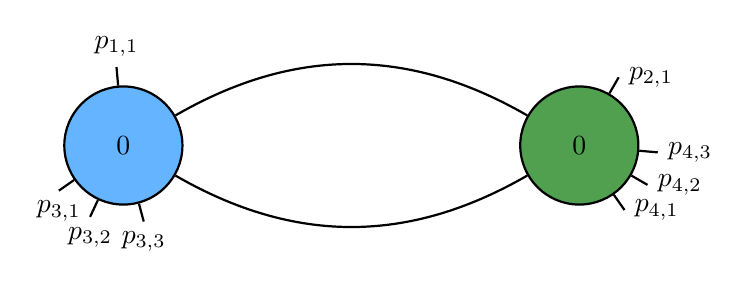
\begin{tikzpicture}[thick,amat/.style={matrix of nodes,nodes in empty cells,
  row sep=3.2em,rounded corners,
  nodes={draw,solid,circle,minimum size=1.5cm}},
  dmat/.style={matrix of nodes,nodes in empty cells,row sep=3.2em,nodes={minimum size=1.5cm},draw=myred},
  fsnode/.style={fill=myblue},
  ssnode/.style={fill=mygreen}]

  \matrix[amat,nodes=fsnode] (mat1) {$0$\\};

 \matrix[amat,right=4cm of mat1,nodes=ssnode] (mat2) {$0$\\};

 \draw  (mat1-1-1) edge[bend left] (mat2-1-1)
 (mat1-1-1) edge[bend right] (mat2-1-1);

  % draw legs for left side
 \draw (mat1-1-1) -- +(95:1) node[anchor=south] {$p_{1,1}$}
 (mat1-1-1) -- +(215:1) node[anchor=north] {$p_{3,1}$}
 (mat1-1-1) -- +(245:1) node[anchor=north] {$p_{3,2}$}
 (mat1-1-1) -- +(285:1) node[anchor=north] {$p_{3,3}$};

 % draw legs for right side
 \draw  (mat2-1-1) -- +(60:1) node[anchor=west] {$p_{2,1}$}
 (mat2-1-1) -- +(305:1) node[anchor=west] {$p_{4,1}$}
 (mat2-1-1) -- +(330:1) node[anchor=west] {$p_{4,2}$}
 (mat2-1-1) -- +(355:1) node[anchor=west] {$p_{4,3}$};

              \end{tikzpicture}

  This is a stable graph $\Gamma$ that specializes to
  $\hat A$ in two ways, by contracting either of
  the two edges; each corresponds to a choice of $\hat A$-structure
  as defined in \cite{Schmitt} (TODO: illustrate what this means).
  In the sense of Definition 2.10 from \cite{Lian}, there is an admissible cover of stable graphs $\Gamma\to\Gamma'$ depicted as follows where $a+b=4$:

                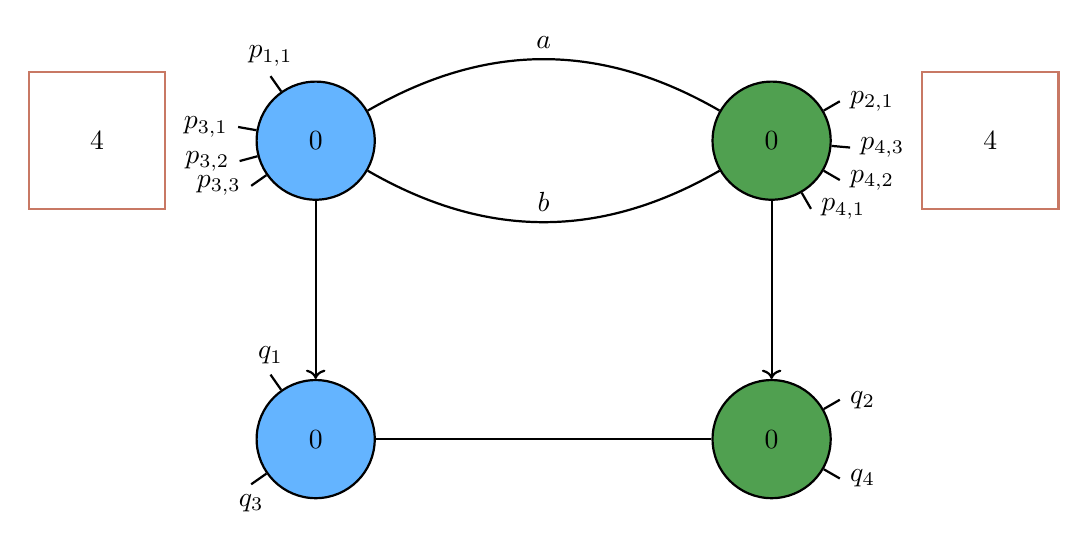
\begin{tikzpicture}[thick,amat/.style={matrix of nodes,nodes in empty cells,
  row sep=3.2em,rounded corners,
  nodes={draw,solid,circle,minimum size=1.5cm}},
  dmat/.style={matrix of nodes,nodes in empty cells,row sep=3.2em,nodes={minimum size=1.5cm},draw=myred},
  fsnode/.style={fill=myblue},
  ssnode/.style={fill=mygreen}]

  \matrix[amat,nodes=fsnode] (mat1) {$0$\\};

    \matrix[dmat,left=1cm of mat1] (degrees1) {$4$\\};


 \matrix[amat,right=4cm of mat1,nodes=ssnode] (mat2) {$0$\\};

 \matrix[dmat,right=1cm of mat2] (degrees2) {$4$\\};

 \draw  (mat1-1-1) edge[bend left,"$a$"] (mat2-1-1)
 (mat1-1-1) edge[bend right,"$b$"] (mat2-1-1);

  % draw legs for left side
 \draw (mat1-1-1) -- +(125:1) node[anchor=south] {$p_{1,1}$}
 (mat1-1-1) -- +(170:1) node[anchor=east] {$p_{3,1}$}
 (mat1-1-1) -- +(195:1) node[anchor=east] {$p_{3,2}$}
 (mat1-1-1) -- +(215:1) node[anchor=east] {$p_{3,3}$};

 % draw legs for right side
 \draw  (mat2-1-1) -- +(30:1) node[anchor=west] {$p_{2,1}$}
 (mat2-1-1) -- +(300:1) node[anchor=west] {$p_{4,1}$}
 (mat2-1-1) -- +(330:1) node[anchor=west] {$p_{4,2}$}
 (mat2-1-1) -- +(355:1) node[anchor=west] {$p_{4,3}$};

 \matrix[amat,nodes=fsnode,below=2cm of mat1] (mat3) {$0$\\};

 \matrix[amat,nodes=ssnode,below=2cm of mat2] (mat4) {$0$\\};

  \draw (mat3-1-1) -- +(125:1) node[anchor=south] {$q_1$}
 (mat3-1-1) -- +(215:1) node[anchor=north] {$q_3$};
   
  \draw  (mat4-1-1) -- +(30:1) node[anchor=west] {$q_2$}
 (mat4-1-1) -- +(330:1) node[anchor=west] {$q_4$};

 \draw  (mat3-1-1) edge[] (mat4-1-1);

 \draw  (mat1-1-1) edge[->] (mat3-1-1);
 \draw  (mat2-1-1) edge[->] (mat4-1-1);

                \end{tikzpicture}

                The contribution of such $(\Gamma,\Gamma')$ is
                \[
                \frac 1{|\Aut(\Gamma)|}c_{\Gamma}W_{(\Gamma,\Gamma')}=\frac 1{|\Aut(a,b)|}\cdot 4\cdot \overline H((4),(a,b),(2,1,1))\cdot \overline H((4),(a,b),(2,1,1))
                \]
                When $(a,b)=(2,2)$ this is
                \[
                \frac 12\cdot 4\cdot 2\cdot 2=8
                \]
                and when $(a,b)=(3,1)$ this is
                \[
                1\cdot 4\cdot 2\cdot 2=16.
                \]
                There are similar choices of $(\Gamma,\Gamma')$ where the components of $q_3$ and
                $q_4$ are swapped,
                yielding a cumulative sum of $2\cdot (8+16)=48$.

                The other type of cover $\Gamma\to\Gamma'$ to consider can be depicted as follows:

                                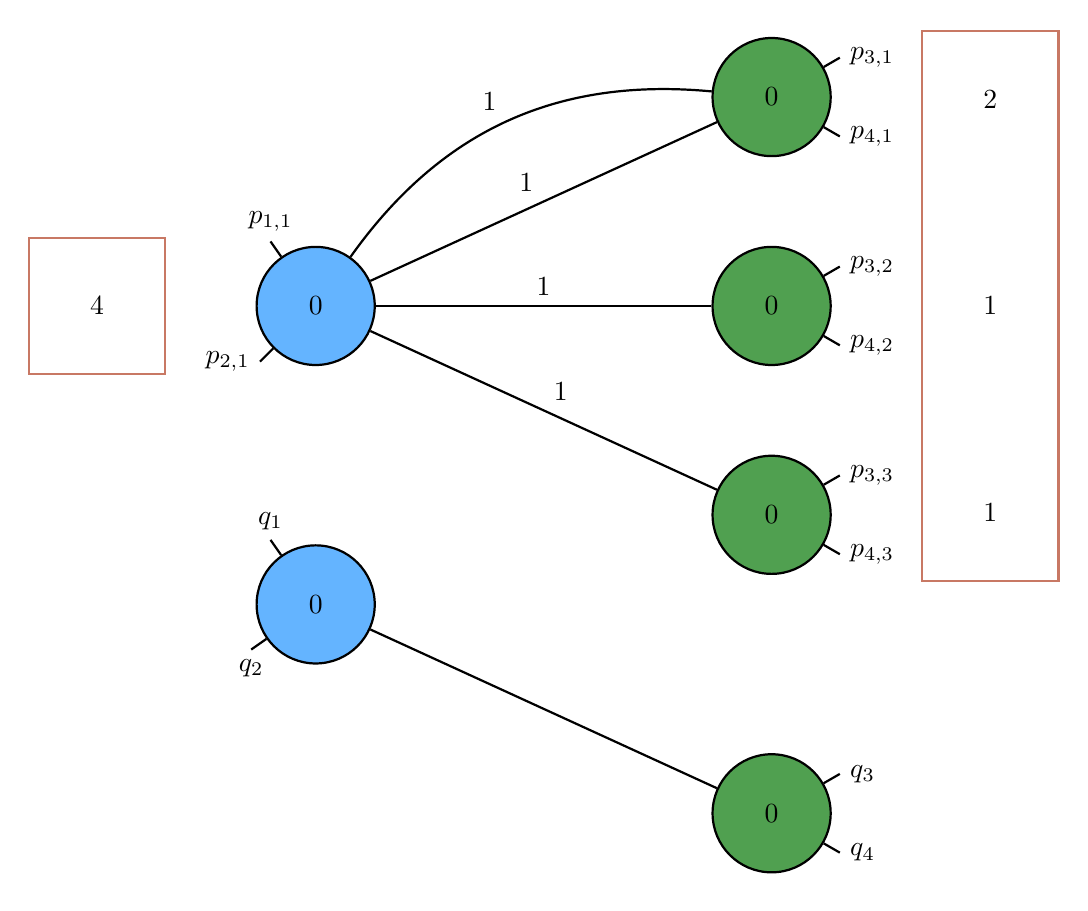
\begin{tikzpicture}[thick,amat/.style={matrix of nodes,nodes in empty cells,
  row sep=3.2em,rounded corners,
  nodes={draw,solid,circle,minimum size=1.5cm}},
  dmat/.style={matrix of nodes,nodes in empty cells,row sep=3.2em,nodes={minimum size=1.5cm},draw=myred},
  fsnode/.style={fill=myblue},
  ssnode/.style={fill=mygreen}]

  \matrix[amat,nodes=fsnode] (mat1) {$0$\\};

    \matrix[dmat,left=1cm of mat1] (degrees1) {$4$\\};


    \matrix[amat,right=4cm of mat1,nodes=ssnode] (mat2) {$0$\\
      $0$\\
    $0$\\};

 \matrix[dmat,right=1cm of mat2] (degrees2) {$2$\\
   $1$\\
 $1$\\};

 \draw  (mat1-1-1) edge[bend left,"$1$"] (mat2-1-1)
 (mat1-1-1) edge["$1$"] (mat2-1-1)
 (mat1-1-1) edge["$1$"] (mat2-2-1)
 (mat1-1-1) edge["$1$"] (mat2-3-1);

  % draw legs for left side
 \draw (mat1-1-1) -- +(125:1) node[anchor=south] {$p_{1,1}$}
 (mat1-1-1) -- +(225:1) node[anchor=east] {$p_{2,1}$};

 % draw legs for right side
 \draw  (mat2-1-1) -- +(30:1) node[anchor=west] {$p_{3,1}$}
 (mat2-2-1) -- +(30:1) node[anchor=west] {$p_{3,2}$}
 (mat2-3-1) -- +(30:1) node[anchor=west] {$p_{3,3}$}
 (mat2-1-1) -- +(330:1) node[anchor=west] {$p_{4,1}$}
 (mat2-2-1) -- +(330:1) node[anchor=west] {$p_{4,2}$}
 (mat2-3-1) -- +(330:1) node[anchor=west] {$p_{4,3}$};

 \matrix[amat,nodes=fsnode,below=2cm of mat1] (mat3) {$0$\\};

 \matrix[amat,nodes=ssnode,below=2cm of mat2] (mat4) {$0$\\};

  \draw (mat3-1-1) -- +(125:1) node[anchor=south] {$q_1$}
 (mat3-1-1) -- +(215:1) node[anchor=north] {$q_2$};
   
  \draw  (mat4-1-1) -- +(30:1) node[anchor=west] {$q_3$}
 (mat4-1-1) -- +(330:1) node[anchor=west] {$q_4$};

 \draw  (mat3-1-1) edge[] (mat4-1-1);

                                \end{tikzpicture}

                                There are $2\cdot 2$ choices for placement of $p_{3,2}$ and $p_{4,2}$
                                and $2\cdot 2$ automorphisms of the graph
                                (swapping the two top edges and swapping
                                the two lower right vertices), so
                                the contribution
                                is
                                \begin{align*}
                                  4\cdot \frac 1{|\Aut(\Gamma)|}c_{\Gamma}W_{(\Gamma,\Gamma')}&=4\cdot\frac 14\cdot 2\cdot \overline H((4),(4),(1,1,1,1))\cdot \overline H((2),(2),(1,1)) \\
                                  &=2\cdot 6\cdot 1\\
                                  &=12
                                \end{align*}
                                Combining our results,
                                \[
                                \frac 12W_{(4),(2,1,1),(2,1,1)}(4)=48+12=60\implies W_{(4),(2,1,1),(2,1,1)}(4)=120\implies N_{(4),(2,1,1),(2,1,1)}(4)=\frac{120}{2^3}=15
                                \]
                                This matches our expectation, since $N_{(4),(2,1,1),(2,1,1)}(4)$ counts
                                nontrivial $4$-torsion points of an elliptic curve.
                                
\end{eg}

In general, any invariant $W_{\sigma_1,\dots,\sigma_n}(d)$ can be computed via this method, using the
same graph $A$ in this example and reducing to genus $0$ invariants (which will all be marked
Hurwitz numbers).

  \subsection{Merging two points}

  In the case where $\ell(\mu)\geq 2$, we can consider the following graph $A$:

                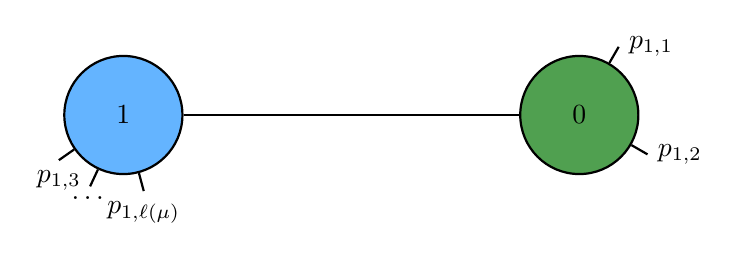
\begin{tikzpicture}[thick,amat/.style={matrix of nodes,nodes in empty cells,
  row sep=3.2em,rounded corners,
  nodes={draw,solid,circle,minimum size=1.5cm}},
  dmat/.style={matrix of nodes,nodes in empty cells,row sep=3.2em,nodes={minimum size=1.5cm},draw=myred},
  fsnode/.style={fill=myblue},
  ssnode/.style={fill=mygreen}]

  \matrix[amat,nodes=fsnode] (mat1) {$1$\\};

 \matrix[amat,right=4cm of mat1,nodes=ssnode] (mat2) {$0$\\};

 \draw  (mat1-1-1) edge (mat2-1-1);

  % draw legs for left side
 \draw (mat1-1-1) -- +(215:1) node[anchor=north] {$p_{1,3}$}
 (mat1-1-1) -- +(245:1) node[anchor=north] {$\dots$}
 (mat1-1-1) -- +(285:1) node[anchor=north] {$p_{1,\ell(\mu)}$};

 % draw legs for right side
 \draw  (mat2-1-1) -- +(60:1) node[anchor=west] {$p_{1,1}$}
 (mat2-1-1) -- +(330:1) node[anchor=west] {$p_{1,2}$};

                \end{tikzpicture}

                By applying the theorem to this graph, we can compute the value of
                $W_{\sigma_1,\dots,\sigma_n}(\mu)$ by reduction to marked Hurwitz
                numbers and terms of the form
                $W_{\tau_1,\dots,\tau_m}(\mu')$ where $\ell(\mu')<\ell(\mu)$, for instance
                in the first example of this section.
                The base case where $\ell(\mu)=1$ can be solved via genus reduction.
                In principle, this gives us a complete (albeit potentially combinatorially difficult) method to compute any invariant $W_{\sigma_1,\dots,\sigma_n}(\mu)$.

                More generally, we can use the theorem to compute $W_{g,\sigma,\nu}$ when $m=\sum\limits_{i=1}^n|\nu_i|\geq 2$, by letting $A$ be a graph with a genus $g$ vertex attached to a genus $0$ vertex, and two of the
                marked points on the genus $0$ vertex. The following lemma will be useful:

                \begin{lem}
                  \label{lem:branchpoints}
                  Letting $A$ be as above, in Theorem~\ref{thm:admissible}, every admissible cover of graphs $\Gamma\to\Gamma'$ where $\Gamma$ contains a genus $g$ vertex (guaranteed when $g=1$) has precisely $2$ branch points
                  whose fiber does not intersect the genus $g$ vertex.
                \end{lem}

                \begin{proof}
                  Let $\Gamma\to\Gamma'$ be an admissible cover of graphs where $\Gamma$ comes with a $\hat A$-structure and $\hat A$ specializes to $A$, and assume $\Gamma$ has a genus $g$ vertex $v$.
                  Then $\Hb_{(\Gamma,\Gamma')}$ has a factor $\Hb_{v}$ corresponding to the vertex $v$,
                  and there is a finite map $\Hb_{v}\to\overline{\mathcal M_{g,m-1}}$ which recalls
                  the vertex $v$ along with the $m-2$ fixed points on the genus $g$ vertex of $A$ and
                  the point corresponding to the node of $A$. Thus,
                  \[
                  \dim(\Hb_v)=\dim(\overline{\mathcal M_{g,m-1}})=3g-3+m-1
                  \]
                  By Equation~\ref{eqn:dimension}, $\dim(\Hb_v)=n-4$. There is also a finite morphism
                  $\Hb_v\to\overline{\mathcal M_{0,k+1}}$ where $k$ is the number of proper branch points from this
                  component (and thus $k+1$ is the number of branch points including the node), so
                  \[
                  k-2=n-4\implies k=n-2
                  \]
                  and therefore the number of branch points not arising from the genus $g$ vertex is $n-(n-2)=2$.
                  \end{proof}


\section{All twos case}

In this section we study the invariants $N_{\mu,(2^k),(2^k)}$ defined for $d=2k$ even.
We will ultimately prove that
\[
N_{\mu,(2^k),(2^k)}=3\cdot 2^{\ell(\mu)-1},
\]
along the way demonstrating techniques to compute our invariants, which will prove the result in special instances.

First, we will translate the calculation of $N_{\mu,(2^k),(2^k)}$ into a problem of intersection theory
in projective space, which we will solve in the special case where $\mu=(1^d)$.
We will then calculate the opposite extreme case, where $\mu=(d)$, first by use of Hurwitz theory and
secondly by a genus reduction technique. Finally, we will establish the result in full generality using
our most powerful technique: establishing a recursion between these invariants by use of
our admissible covers technique, which yields the full solution in combination with either of the base
cases we have computed.

\subsection{Motivation}

The Gromov-Witten invariants of an elliptic curve are well understood. However, a natural generalization
remains open: let $C$ be the quotient of an elliptic curve under the action $x\mapsto -x$.
This action has $4$ fixed points (the two-torsion points in the group law), and so as an orbifold
$C$ can be identified as $\P^1$ with $4$ points of stabilizer $\Z/2$, and is known as the
{\it pillowcase orbifold}. Maps $E\to C$ correspond to maps $E\to\P^1$ with ``even'' ramification over
the $4$ special points, and so $N_{\mu,(2^k),(2^k)}$ can be interpreted as a relative Gromov-Witten
invariant of the pillowcase $C$, fitting into a larger picture of classes $\langle \mu\rangle_d^{C}\in H^{g-1}(\overline{\mathcal M}_{g,\ell(\mu)})$.

\subsection{Geometric interpretation}

The problem can be restated in geometric terms as follows: let $E\subset \P^{d-1}$ be a general genus $1$ curve,
and let $H_0$ be a general hyperplane such that $H_0\cap E$ has type $\mu$. Then letting \[X_{(2^k)}=\{H\in(\P^{d-1})^*:H\cap E\text{ is of type }(2^k)\}\]
and $\pi:(\P^{d-1})^*\dashrightarrow \P^{d-2}$ be projection away from $H_0$, we want the number of fibers of $\pi$
containing multiple points of $X_{(2^k)}$.

For any $H\in X_{(2^k)}$, we know $H\cap E=2p_1+\dots+2p_k$ for some points $p_1,\dots,p_k\in E$. Then in the group law, we have
\[
2p_1+\dots+2p_k=0\implies p_1+\dots+p_k\in\{t_1,t_2,t_3,t_4\}
\]
where the $t_i$ are the $2$-torsion points of $E$. This means we have a map $X_{(2^k)}\to\{t_1,t_2,t_3,t_4\}$ sending $H\mapsto p_1+\dots+p_k$, and since the target is discrete, $X_{(2^k)}$ can be divided into four connected components:
\[
X_{(2^k)}=X_{(2^k)}^{(1)}\cup X_{(2^k)}^{(2)}\cup X_{(2^k)}^{(3)}\cup X_{(2^k)}^{(4)}
\]
Each component is (abstractly? TODO) isomorphic to $E^{k-1}/\sim\cong \P^{k-1}$,
and our goal is to count the size of $\pi(X_{(2^k)}^{(i)})\cap \pi(X_{(2^k)}^{(j)})$
for $i\neq j$.

It will be necessary to compute the degree of $X_{(2^k)}$, so we begin with a more general calculation of the degree of $X_{\mu}$:

\begin{lem}
  If $\mu=(\mu_1,\dots,\mu_n)$ with $|\mu|=d$, then
  \[
  \text{deg}(X_{\mu})=\frac{\mu_1\cdots\mu_n\cdot d(n-1)!}{|\text{Aut}(\mu)|}
  \]
\end{lem}

\begin{proof}
  We use Proposition 5.1, p 358 of ``Geometry of Algebraic Curves'' by Arbarello, Cornalba, Griffiths and Harris. Considering the map
  $\phi:E^n\to\text{Sym}^dE$ sending $(x_1,\dots,x_n)\mapsto \sum_{i=1}^n\mu_ix_i$,
  the degree we want is the restriction of $x^{n-1}[\text{im}(\phi)]$ to
  the divisor $(\P^{d-1})^*\subset\text{Sym}^dE$ consisting of effective divisors
  equivalent to our given divisor. We know that $\theta$ vanishes when
  restricted to our $(\P^{d-1})^*$, so we only need consider the case $\alpha=\beta=0$ in the Proposition and
  \begin{align*}
    \phi_*[E^n]x^{n-1}\bigg|_{(\P^{d-1})^*}&=[(1+\mu_1t_1+\dots+\mu_nt_n)^{n-1}(1+\mu_1^2t_1+\dots+\mu_n^2t_n)]_{t_1\cdots t_n}\\
    &=\sum_{i=1}^n(n-1)!(\mu_1\cdots\hat{\mu_i}\cdots \mu_n)\cdot\mu_i^2\\
    &=(n-1)!\mu_1\cdots\mu_n\cdot (\mu_1+\dots+\mu_n)
  \end{align*}

  
  The map $\phi$ is $|\Aut(\mu)|$-to-1, and so we end up with our result.
  \end{proof}
In particular,
\[
\text{deg}(X_{(2^k)})=\frac{(k-1)!2^k(2k)}{k!}=2^{k+1}\implies \text{deg}(X_{(2^k)}^{(i)})=2^{k-1}.
\]
Let $\mu=(1^{d})$. Then the intersection is the sum of product of degrees of $X_{(2^k)}^{(i)}$ and $X_{(2^k)}^{(j)}$ for $i\neq j$, i.e.
\[
\binom 42\cdot 2^{k-1}\cdot 2^{k-1}=6\cdot 2^{d-2}=3\cdot 2^{d-1}
\]
in agreement with our main claim.


\subsection{$\mu=(d)$}

Having proved the result geometrically for $\mu=(1,\dots,1)$, we now tackle the other extreme case, where $\mu=(d)$. We will show that $N_{(d),(2^k),(2^k)}=3$
using two methods: first, by categorizing all such maps explicitly using Hurwitz theory and counting them, and second by performing a genus reduction.

\subsubsection{Combinatorial solution}

\begin{figure}[h]
  \caption{Factored Hurwitz cover with even ramification, in the case where $k$ is odd}
  \centering
\begin{tikzpicture}
  \draw[domain=-6:7.5,samples=50,color=gray!50,thick] plot (\x, \x^3/64 - \x/2); % Curve E
  \draw[domain=-6:7.5,samples=50,color=gray!50,thick] plot (\x, -4); % first P^1
  \draw[domain=-6:7.5,samples=50,color=gray!50,thick] plot (\x, -8); % second P^1

  % top map arrows and labels
  \foreach \p/\plabel/\qlabel in {-5/$p$/$q_1$, -1//$q_2$, 3//$q_3$, 7//$q_4$} {
    \filldraw[black] (\p, \p^3/64-\p/2) circle (0.6mm) node[above] {\plabel};
    \draw[->] (\p, \p^3/64-\p/2-.4) to["2"] (\p, -3.5);
    \filldraw[black] (\p, -4) circle (0.6mm) node[below] {\qlabel};
  }

  % fiber over 0
  \draw[->] (-5, -4.5) to["$k$"] (-5, -7.5);

  % fiber over 1
  \foreach \x/\l in {-4/$2$, -3/$\dots$, -2/$2$, -1/$1$} {
    \draw[->] (\x, -4.5) to["\l"] (-3/2+\x/4, -7.5);
  }

    % fiber over infinity
  \foreach \x/\l in {0/$2$, 1/$\dots$, 2/$2$, 3/$1$} {
    \draw[->] (\x, -4.5) to["\l"] (3/2+\x/4, -7.5);
  }

  % fiber over w
  \foreach \x/\l in {4/$1$, 5/$1$, 6/$\dots$, 7/$1$} {
    \draw[->] (\x, -4.5) to["\l"] (9/2+\x/4, -7.5);
  }

  % 0, 1, infinity, w
  \foreach \x/\l in {-5/$0$, -2/$1$, 2/$\infty$, 6/$w$} {
    \filldraw[black] (\x, -8) circle (0.6mm) node[below] {\l};
    }

\end{tikzpicture}

\label{fig:comb1}
\end{figure}

\begin{figure}[h]
  \caption{Factored Hurwitz cover with even ramification, in the case where $k$ is even}
  \centering
\begin{tikzpicture}
  \draw[domain=-6:7.5,samples=50,color=gray!50,thick] plot (\x, \x^3/64 - \x/2); % Curve E
  \draw[domain=-6:7.5,samples=50,color=gray!50,thick] plot (\x, -4); % first P^1
  \draw[domain=-6:7.5,samples=50,color=gray!50,thick] plot (\x, -8); % second P^1

  % top map arrows and labels
  \foreach \p/\plabel/\qlabel in {-5/$p$/$q_1$, -4//$q_2$, -3//$q_3$, 5//$q_4$} {
    \filldraw[black] (\p, \p^3/64-\p/2) circle (0.6mm) node[above] {\plabel};
    \draw[->] (\p, \p^3/64-\p/2-.4) to["2"] (\p, -3.5);
    \filldraw[black] (\p, -4) circle (0.6mm) node[below] {\qlabel};
  }

  % fiber over 0
  \draw[->] (-5, -4.5) to["$k$"] (-5, -7.5);

  % fiber over 1
  \foreach \x/\l in {-4/$1$, -3/$1$, -2/$2$, -1/$\dots$, 0/$2$} {
    \draw[->] (\x, -4.5) to["\l"] (-3/2+\x/4, -7.5);
  }

    % fiber over infinity
  \foreach \x/\l in {1/$2$, 2/$\dots$, 3/$2$} {
    \draw[->] (\x, -4.5) to["\l"] (3/2+\x/4, -7.5);
  }

  % fiber over w
  \foreach \x/\l in {5/$1$, 6/$\dots$, 7/$1$} {
    \draw[->] (\x, -4.5) to["\l"] (9/2+\x/4, -7.5);
  }

  % 0, 1, infinity, w
  \foreach \x/\l in {-5/$0$, -2/$1$, 2/$\infty$, 6/$w$} {
    \filldraw[black] (\x, -8) circle (0.6mm) node[below] {\l};
    }

\end{tikzpicture}

\label{fig:comb2}
\end{figure}

%\includegraphics[scale=0.2]{diagram.jpg}

%\includegraphics[angle=90,scale=0.15]{diagram2.jpg}

\begin{claim}
  Let $f:E\to\P^1$ be of degree $d=2k$ such that $f(p)=0$ with full ramification,
  and $f$ has ramification profiles $(2^k)$ over $1$ and $\infty$. Then $f$ factors as
  $E\to\P^1\to\P^1$ where the first map is degree $2$ and the second is degree $k$.
\end{claim}
\begin{proof}
  Figures \ref{fig:comb1} and \ref{fig:comb2} illustrate how such maps should factor. We prove the claim by fixing branch points $0,1,\infty,w$ in $\P^1$, counting the (orbifold) number of factored
  maps over these branch points as well as the maps in Figure \ref{fig:twos}, and showing that these are equal.

\begin{figure}[h]
  \caption{Hurwitz covers with even ramification}
  \centering
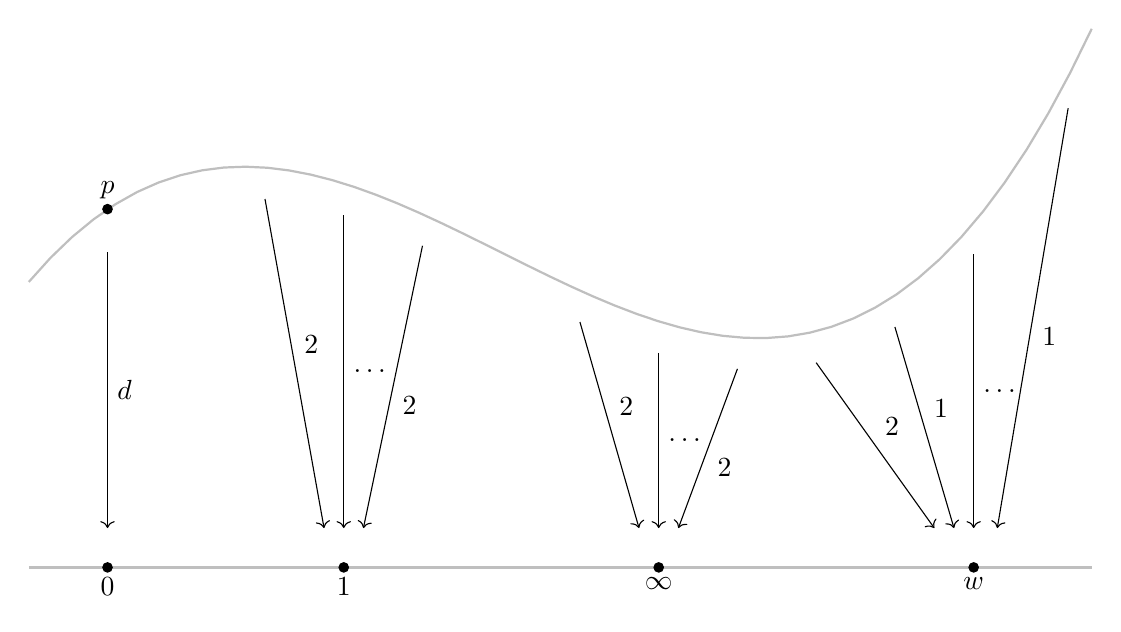
\begin{tikzpicture}
  \draw[domain=-6:7.5,samples=50,color=gray!50,thick] plot (\x, \x^3/64 - \x/2); % Curve E
  \draw[domain=-6:7.5,samples=50,color=gray!50,thick] plot (\x, -4); % P^1

  \filldraw[black] (-5, .55) circle (0.6mm) node[above] {$p$};

  % fiber over 0
  \draw[->] (-5, 0) to["$d$"] (-5, -3.5);

  % fiber over 1
  \foreach \x/\l in {-3/$2$, -2/$\dots$, -1/$2$} {
    \draw[->] (\x, \x^3/64-\x/2-.4) to["\l"] (-3/2+\x/4, -3.5);
  }

    % fiber over infinity
  \foreach \x/\l in {1/$2$, 2/$\dots$, 3/$2$} {
    \draw[->] (\x, \x^3/64-\x/2-.4) to["\l"] (3/2+\x/4, -3.5);
  }

  % fiber over w
  \foreach \x/\l in {4/$2$, 5/$1$, 6/$\dots$, 7.2/$1$} {
    \draw[->] (\x, \x^3/64-\x/2-.4) to["\l"] (9/2+\x/4, -3.5);
  }

  % 0, 1, infinity, w
  \foreach \x/\l in {-5/$0$, -2/$1$, 2/$\infty$, 6/$w$} {
    \filldraw[black] (\x, -4) circle (0.6mm) node[below] {\l};
    }

\end{tikzpicture}

\label{fig:twos}
\end{figure}

  The latter count is given by
  \[
  H((d),(2^k),(2^k),(2,1,\dots,1))
  \]
  which is $k/2$ by the Appendix. For the former count, we
  first consider maps $\P^1\to\P^1$  (with $0,1,\infty,w$ fixed)
  described in Figure \ref{fig:comb1} or \ref{fig:comb2} (depending on the parity of $k$). These
  are counted by
  $H((k),(2^{(k-1)/2},1),(2^{(k-1)/2},1))$ if $k$ is odd or
  $H((k),(2^{k/2-1},1,1),(2^{k/2}))$ if $k$ is even, both of which are $1$
  by results of the Appendix. The count for the upstairs map $E\to\P^1$ is
  $H((2),(2),(2),(2))=\frac 12$ multiplied by the number of options for point $q_4$
  (which is $k$). Thus, the orbifold number of factored maps lying over $0,1,\infty,w$ is $1\cdot \frac 12\cdot k$, proving the claim.
  
\end{proof}

Now given this result, we can compute $N_{(2^k),(2^k)}(d)$ by counting
the number of factored maps described in Figures \ref{fig:comb1} and \ref{fig:comb2} for a fixed $(E,p)$.
The map $(E,p)\to(\P^1,q_1)$ is the elliptic map to $\P^1$ and therefore unique up
to automorphisms of $\P^1$ fixing $q_1$; there are $3$ choices for the point
$q_4$, and after this the map is uniquely determined up to automorphisms of
$\P^1$ (by the Hurwitz counts above). Therefore,
\[
N_{(2^k),(2^k)}(d)=3.
\]

\subsubsection{Genus reduction}

We apply the method of Section 3 to yield another proof that
$N_{(2^k),(2^k)}(d)=3$:

\begin{claim}
  For $d=2k$ even,
  \[
  W_{(2^k),(2^k),(2,1^{d-2})}(d)=6(d-2)!\cdot (k!)^2
  \]
\end{claim}
\begin{proof}
  Let $A$ be a stable graph consisting of a genus $0$ vertex with a loop and a marked point $p_{1,1}$.
  Let $\hat A$ be the stable graph with additional marked points on the genus $0$ vertex for
  the further ramification.

There are two kinds of
admissible covers $\Gamma\to\Gamma'$ with $\Gamma$ specializing to $\hat A$. The first
is of the form:

            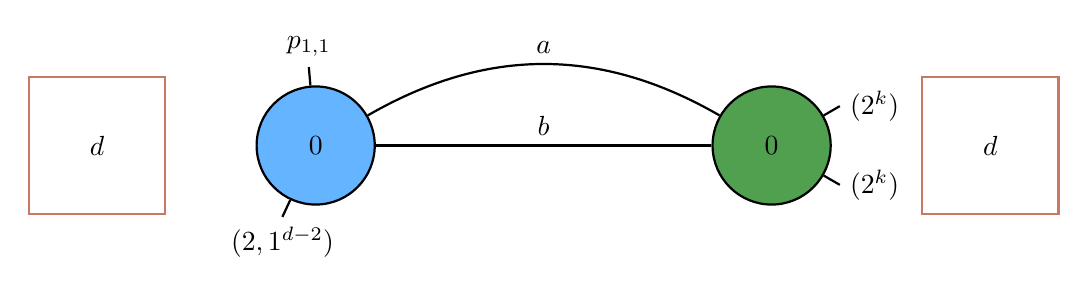
\begin{tikzpicture}[thick,amat/.style={matrix of nodes,nodes in empty cells,
  row sep=3.2em,rounded corners,
  nodes={draw,solid,circle,minimum size=1.5cm}},
  dmat/.style={matrix of nodes,nodes in empty cells,row sep=3.2em,nodes={minimum size=1.5cm},draw=myred},
  fsnode/.style={fill=myblue},
  ssnode/.style={fill=mygreen}]

  \matrix[amat,nodes=fsnode] (mat1) {$0$\\};

    \matrix[dmat,left=1cm of mat1] (degrees1) {$d$\\};


 \matrix[amat,right=4cm of mat1,nodes=ssnode] (mat2) {$0$\\};

 \matrix[dmat,right=1cm of mat2] (degrees2) {$d$\\};

 \draw  (mat1-1-1) edge["$a$",bend left] (mat2-1-1)
 (mat1-1-1) edge["$b$"] (mat2-1-1);

  % draw legs for left side
 \draw (mat1-1-1) -- +(95:1) node[anchor=south] {$p_{1,1}$}
 (mat1-1-1) -- +(245:1) node[anchor=north] {$(2,1^{d-2})$};

 % draw legs for right side
 \draw  (mat2-1-1) -- +(30:1) node[anchor=west] {$(2^k)$}
 (mat2-1-1) -- +(330:1) node[anchor=west] {$(2^k)$};

            \end{tikzpicture}

            There are two $\hat A$-structures, corresponding to a choice
            of edge to contract, and so $c_{\Gamma}=a+b=d$. The right-hand count here under Theorem~\ref{thm:admissible} is
            \begin{align*}
              \overline H((d),(a,b),(2,1^{d-2}))\cdot \overline H((2^k),(2^k),(a,b))\cdot d\cdot\frac 1{|\Aut(a,b)|}
            \end{align*}
            By Claim TODO in Appendix 1, the second term vanishes unless $a=b=k$, in which case
            the count (by Claims TODO and TODO) is
            \[
            (1\cdot (d-2)!)\cdot \left(\frac 1d\cdot k!\cdot k!\cdot 2\right)\cdot d\cdot\frac 12
            =(d-2)!\cdot (k!)^2
            \]

            Now the second picture is of the form:
            
            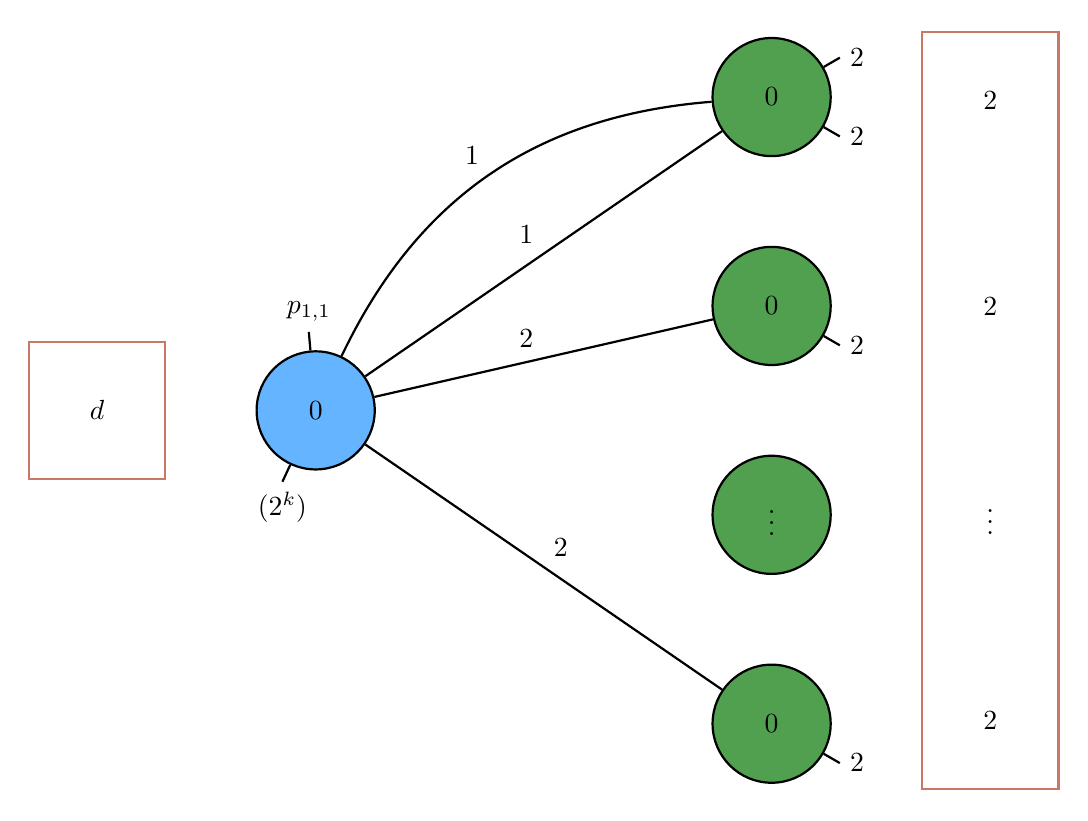
\begin{tikzpicture}[thick,amat/.style={matrix of nodes,nodes in empty cells,
  row sep=3.2em,rounded corners,
  nodes={draw,solid,circle,minimum size=1.5cm}},
  dmat/.style={matrix of nodes,nodes in empty cells,row sep=3.2em,nodes={minimum size=1.5cm},draw=myred},
  fsnode/.style={fill=myblue},
  ssnode/.style={fill=mygreen}]

  \matrix[amat,nodes=fsnode] (mat1) {$0$\\};

    \matrix[dmat,left=1cm of mat1] (degrees1) {$d$\\};


 \matrix[amat,right=4cm of mat1,nodes=ssnode] (mat2) {$0$\\
      $0$\\
      $\vdots$\\
  $0$\\};

 \matrix[dmat,right=1cm of mat2] (degrees2) {$2$\\
   $2$ \\
    \vdots \\
    $2$\\};

 \draw  (mat1-1-1) edge["$1$",bend left] (mat2-1-1)
 (mat1-1-1) edge["$1$"] (mat2-1-1)
 (mat1-1-1) edge["$2$"] (mat2-2-1)
 (mat1-1-1) edge["$2$"] (mat2-4-1);

  % draw legs for left side
 \draw (mat1-1-1) -- +(95:1) node[anchor=south] {$p_{1,1}$}
 (mat1-1-1) -- +(245:1) node[anchor=north] {$(2^k)$};

 % draw legs for right side
 \draw  (mat2-1-1) -- +(30:1) node[anchor=west] {$2$}
 (mat2-1-1) -- +(330:1) node[anchor=west] {$2$}
 (mat2-2-1) -- +(330:1) node[anchor=west] {$2$}
 (mat2-4-1) -- +(330:1) node[anchor=west] {$2$};

            \end{tikzpicture}

            With markings remembered, the number of such diagrams is
            \[
            2\cdot k\cdot\binom{d-2}{2}\cdot\binom{d-4}{2}\cdot\dots\cdot\binom 22=2k\cdot\frac{(d-2)!}{2^{k-1}}
            \]
            There are two $\hat A$-structures, each with associated coefficient $2^{k-1}$,
            and so the combined contribution to the right-hand side of Theorem~\ref{thm:admissible} is
            \begin{align*}
              &2k\cdot\frac{(d-2)!}{2^{k-1}}\cdot\overline H((d),(2^k),(2^{k-1},1,1))\cdot \overline H((1,1),(2),(2))\cdot \overline H((2),(2),(1,1))^{k-1}\cdot\frac 12\cdot 2\cdot 2^{k-1} \\
              &=2k\cdot (d-2)!\cdot (k!\cdot (k-1)!) \\
              &=2(d-2)!\cdot (k!)^2
            \end{align*}
            We conclude by adding up and seeing that the right-hand side of Theorem~\ref{thm:admissible} is
            \[
            (d-2)!\cdot (k!)^2+ 2(d-2)!\cdot (k!)^2=3(d-2)!\cdot (k!)^2\implies W_{(2^k),(2^k),(2,1^{d-2})}(d)=6(d-2)!\cdot (k!)^2.
            \]

\end{proof}

\subsection{Recursion and general solution}



\section{$S_{\a,\b}$}

\subsection{Definitions and basic results}

Let
\[
S_{\a,\b}(\mu)=
N_{\mu,(2,1,\dots)^{a_2},(2,1,\dots)^{b_2},(3,1,\dots)^{a_3},(3,1,\dots)^{b_3},\dots}^{\{2^{b_2}3^{b_3}\dots\}}
\]
(TODO: fix notation to be consistent with earlier.)
Here $a_2,a_3,\dots$ describe unmarked ramification and $b_2,b_3,\dots$ describe marked ramification. For
simplicity, assume that all ramification is included and define $S_{\mathfrak a,\mathfrak b}(\mu)= 0$ if $\mu_i\leq 0$ for any $i$.

\begin{lem}
  If $S_{\mathfrak a,\mathfrak b}(\mu)$ is well-defined, $|\mathfrak a|=|\mu|+2$.
\end{lem}
\begin{proof}
  Let $\mathcal X$ be the moduli space of maps from a genus $1$ curve to $\mathbb P^1$, with ramification as required for $S_{\mathfrak a,\mathfrak b}(\mu)$, and with all relevant points of the genus $1$ curve marked
  (corresponding to $\mathfrak a$, $\mathfrak b$, and $\mu$). There is a map $\mathcal X\to\overline{\mathcal M}_{1,|\mathfrak b|+|\mu|}$ remembering the genus $1$ curve and the fixed points, which is finite by assumption, so $\dim(\mathcal X)=|\mathfrak b|+|\mu|$. There is also a map $\mathcal X\to\overline{\mathcal M}_{0,|\mathfrak a|+|\mathfrak b|+1}$ remembering the branch points of the target, which is finite by Hurwitz's theorem, and so
  \[
  |\mathfrak b|+|\mu|=\dim(\overline{\mathcal M}_{0,|\mathfrak a|+|\mathfrak b|+1})=|\mathfrak a|+|\mathfrak b|-2
  \]
  yielding the result.
\end{proof}

\subsection{Reduction of $\b$}
\begin{claim}[Claim 1]
  For $n>0$, if $b_y>0$, then
  \begin{align*}
    S_{\mathfrak a,\mathfrak b+\{y\}}(\mu, n) &=S_{\mathfrak a,\mathfrak b}(\mu, n-y+1) +\sum_{z\in\mathfrak a}\min(z-1,y-1,n,y+z-n-2)S_{\mathfrak a-\{z\},\mathfrak b+\{y+z-n-2\}}(\mu)
  \end{align*}
\end{claim}

\begin{proof}
  We consider diagrams which stabilize to a genus $1$ curve containing $x_1,\dots,x_k$ and all but one
  of the other fixed points, attached to a genus $0$ tail containing $q$ (with ramification $n$) and $p$
  (with ramification $y$). Recall by Lemma~\ref{lem:branchpoints} that there are two branch points not
  arising from the genus $1$ component.
  
  A diagram with $x_1,\dots,x_k$ on the right side looks like:

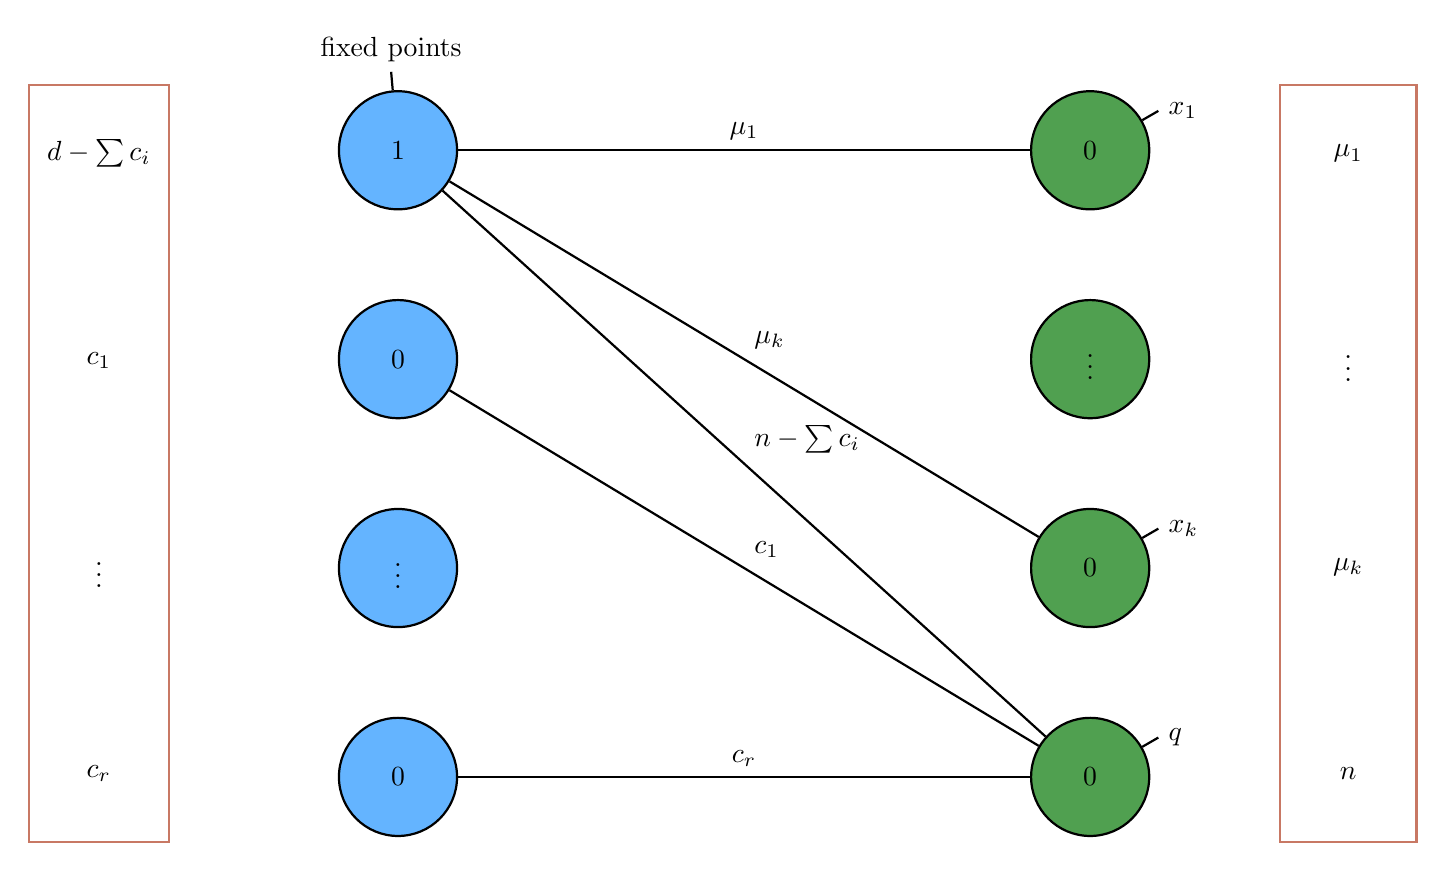
\begin{tikzpicture}[thick,amat/.style={matrix of nodes,nodes in empty cells,
  row sep=3.2em,rounded corners,
  nodes={draw,solid,circle,minimum size=1.5cm}},
  dmat/.style={matrix of nodes,nodes in empty cells,row sep=3.2em,nodes={minimum size=1.5cm},draw=myred},
  fsnode/.style={fill=myblue},
  ssnode/.style={fill=mygreen}]

  \matrix[amat,nodes=fsnode] (mat1) {$1$\\
    $0$\\
    \vdots \\
  $0$\\};

  \matrix[dmat,left=2cm of mat1] (degrees1) {$d-\sum c_i$\\
    $c_1$\\
    \vdots \\
  $c_r$\\};

 \matrix[amat,right=7cm of mat1,nodes=ssnode] (mat2) {$0$\\
   \vdots\\
   $0$ \\
   $0$\\};
 \matrix[dmat,right=1.5cm of mat2] (degrees2) {$\mu_1$\\
   \vdots\\
   $\mu_k$ \\
 $n$\\};

 \draw  (mat1-1-1) edge["$\mu_1$"] (mat2-1-1)
 (mat1-1-1) edge["$\mu_k$"] (mat2-3-1)
 (mat1-1-1) edge["$n-\sum c_i$"] (mat2-4-1)
 (mat1-2-1) edge["$c_1$"] (mat2-4-1)
 (mat1-4-1) edge["$c_r$"] (mat2-4-1);

  % draw legs for left side
 \draw (mat1-1-1) -- +(95:1) node[anchor=south] {fixed points};

 % draw legs for right side
 \draw  (mat2-1-1) -- +(30:1) node[anchor=west] {$x_1$}
 (mat2-3-1) -- +(30:1) node[anchor=west] {$x_k$}
 (mat2-4-1) -- +(30:1) node[anchor=west] {$q$};

\end{tikzpicture}

There are two branch points outside the genus $1$ component, which must be the images of
$x_1,\dots,x_k,q$ and of $p$. This means there is no extra ramification on any genus $0$ component, which is why each top right bubble
connects only to the genus $1$ component. The bottom right bubble must have some ramification beyond what is pictured here, which is necessarily
$p$. So our diagram looks like:

  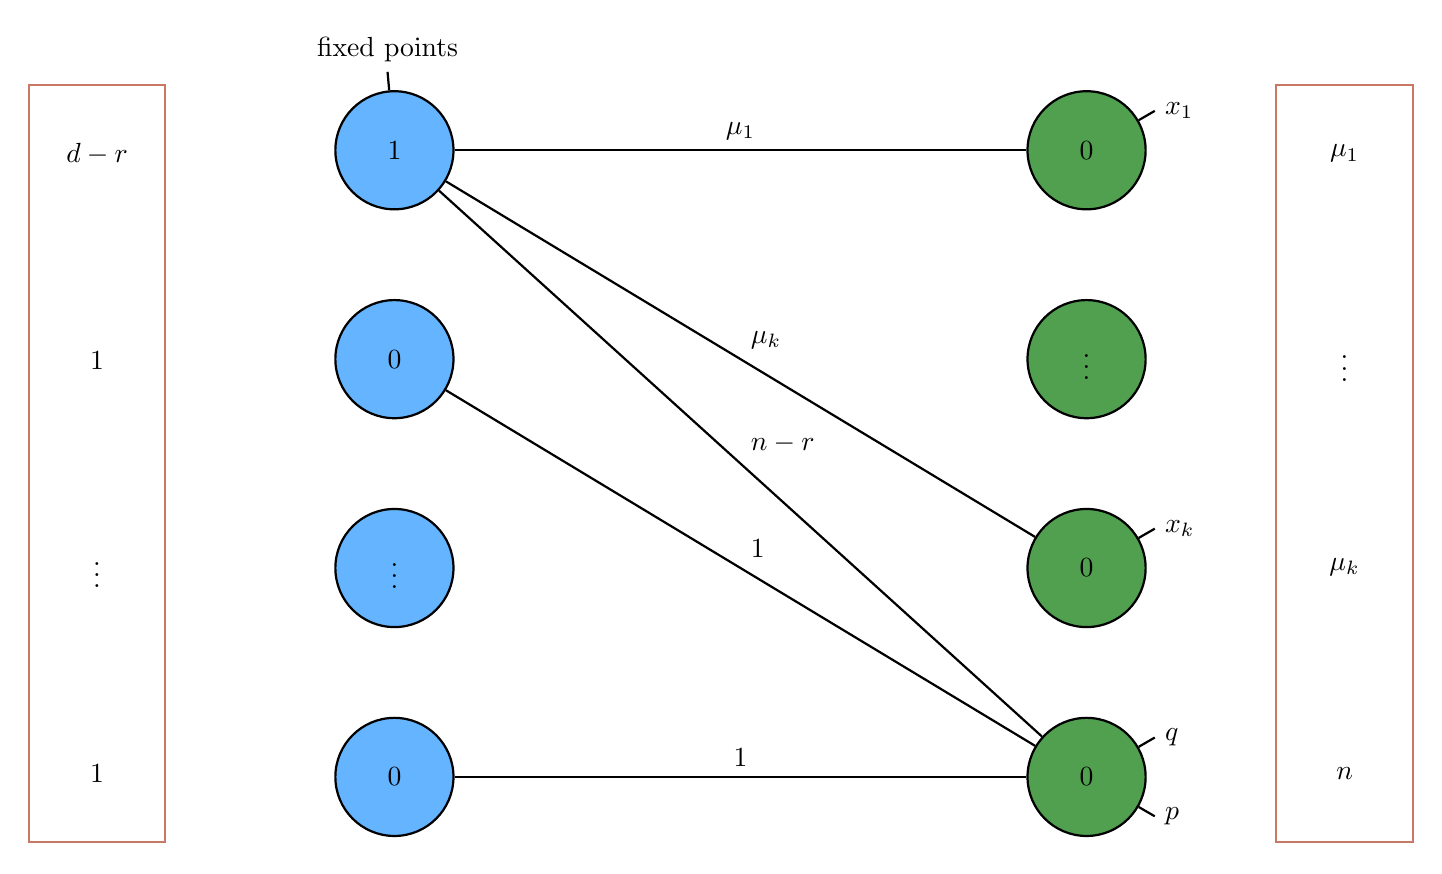
\begin{tikzpicture}[thick,amat/.style={matrix of nodes,nodes in empty cells,
  row sep=3.2em,rounded corners,
  nodes={draw,solid,circle,minimum size=1.5cm}},
  dmat/.style={matrix of nodes,nodes in empty cells,row sep=3.2em,nodes={minimum size=1.5cm},draw=myred},
  fsnode/.style={fill=myblue},
  ssnode/.style={fill=mygreen}]

  \matrix[amat,nodes=fsnode] (mat1) {$1$\\
    $0$\\
    \vdots \\
  $0$\\};

  \matrix[dmat,left=2cm of mat1] (degrees1) {$d-r$\\
    $1$\\
    \vdots \\
  $1$\\};

 \matrix[amat,right=7cm of mat1,nodes=ssnode] (mat2) {$0$\\
   \vdots\\
   $0$ \\
   $0$\\};
 \matrix[dmat,right=1.5cm of mat2] (degrees2) {$\mu_1$\\
   \vdots\\
   $\mu_k$ \\
 $n$\\};

 \draw  (mat1-1-1) edge["$\mu_1$"] (mat2-1-1)
 (mat1-1-1) edge["$\mu_k$"] (mat2-3-1)
 (mat1-1-1) edge["$n-r$"] (mat2-4-1)
 (mat1-2-1) edge["$1$"] (mat2-4-1)
 (mat1-4-1) edge["$1$"] (mat2-4-1);

  % draw legs for left side
 \draw (mat1-1-1) -- +(95:1) node[anchor=south] {fixed points};

 % draw legs for right side
 \draw  (mat2-1-1) -- +(30:1) node[anchor=west] {$x_1$}
 (mat2-3-1) -- +(30:1) node[anchor=west] {$x_k$}
 (mat2-4-1) -- +(30:1) node[anchor=west] {$q$}
 (mat2-4-1) -- +(330:1) node[anchor=west] {$p$};

  \end{tikzpicture}

  As there is no extra ramification outside the genus $1$ component,
  the dimension reduction of $r$ should match the codimension reduction
  corresponding to the removal of $p$, which is $y-1$. So $r=y-1$ and we
  have the first term in the claim, since $H((n),(y,1,\dots),(n-y+1,1,\dots))=1$.

  Now consider the case where $x_1,\dots,x_k,q$ are on the left side. In this
  case, the branch points not coming from the genus $1$ component will be
  the image of $p$ and the image of another point $p'$ (with ramification index $z\in\mathfrak a$). Consider the possibility that
  $x_1,\dots,x_k$ are not all on the genus $1$ component:

  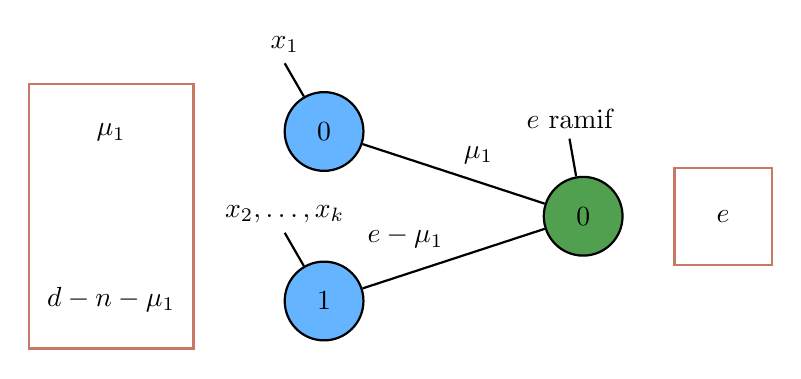
\begin{tikzpicture}[thick,amat/.style={matrix of nodes,nodes in empty cells,
  row sep=3.2em,rounded corners,
  nodes={draw,solid,circle,minimum size=1cm}},
  dmat/.style={matrix of nodes,nodes in empty cells,row sep=3.2em,nodes={minimum size=1cm},draw=myred},
  fsnode/.style={fill=myblue},
  ssnode/.style={fill=mygreen}]

    \matrix[amat,nodes=fsnode] (mat1) {$0$\\
      $1$\\};

    \matrix[amat,right=2cm of mat1,nodes=ssnode] (mat2) {$0$\\};

      \matrix[dmat,left=1cm of mat1] (degrees1) {$\mu_1$\\
    $d-n-\mu_1$\\};

            \matrix[dmat,right=0.5cm of mat2] (degrees2) {$e$\\};
  
 \draw  (mat1-1-1) edge["$\mu_1$"] (mat2-1-1)
 (mat1-2-1) edge["$e-\mu_1$"] (mat2-1-1);

  % draw legs for left side
 \draw (mat1-1-1) -- +(120:1) node[anchor=south] {$x_1$}
 (mat1-2-1) -- +(120:1) node[anchor=south] {$x_2,\dots,x_k$};

   % draw legs for right side
 \draw (mat2-1-1) -- +(100:1) node[anchor=south] {$e$ ramif};


  \end{tikzpicture}

  This would require the genus $0$ on the right side to have multiple branch points contributing
  $e$ ramification,
  but $p$ cannot live on this component (because of the stabilization condition), a contradiction.
  Therefore, $x_1,\dots,x_k$ all live on the genus $1$ component.

  The points $p$ and $p'$ cannot lie on separate components, because the following diagram cannot be completed:

        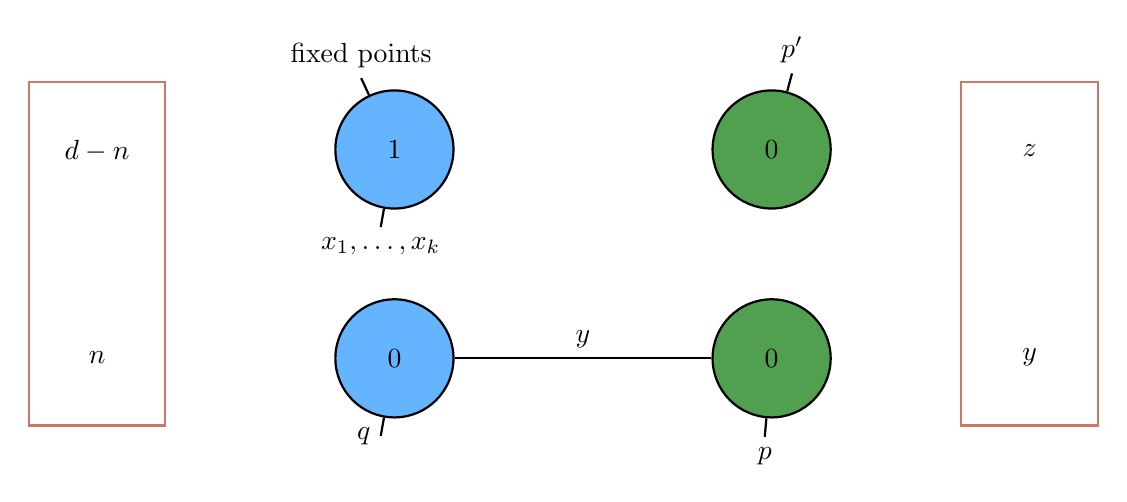
\begin{tikzpicture}[thick,amat/.style={matrix of nodes,nodes in empty cells,
  row sep=3.2em,rounded corners,
  nodes={draw,solid,circle,minimum size=1.5cm}},
  dmat/.style={matrix of nodes,nodes in empty cells,row sep=3.2em,nodes={minimum size=1.5cm},draw=myred},
  fsnode/.style={fill=myblue},
  ssnode/.style={fill=mygreen}]

  \matrix[amat,nodes=fsnode] (mat1) {$1$\\
    $0$\\};

  \matrix[dmat,left=2cm of mat1] (degrees1) {$d-n$\\
    $n$\\};

 \matrix[amat,right=3cm of mat1,nodes=ssnode] (mat2) {$0$\\
   $0$\\};
 \matrix[dmat,right=1.5cm of mat2] (degrees2) {$z$\\
   $y$\\};

 \draw  (mat1-2-1) edge["$y$"] (mat2-2-1);

  % draw legs for left side
 \draw (mat1-1-1) -- +(115:1) node[anchor=south] {fixed points}
 (mat1-1-1) -- +(260:1) node[anchor=north] {$x_1,\dots,x_k$}
 (mat1-2-1) -- +(260:1) node[anchor=east] {$q$};

   % draw legs for right side
 \draw (mat2-1-1) -- +(75:1) node[anchor=south] {$p'$}
 (mat2-2-1) -- +(265:1) node[anchor=north] {$p$};


 \end{tikzpicture}

  Therefore $p$ and $p'$ lie on the same genus $0$ component, all other genus $0$ components on the right side have degree $1$,
  and we end up with:
  
        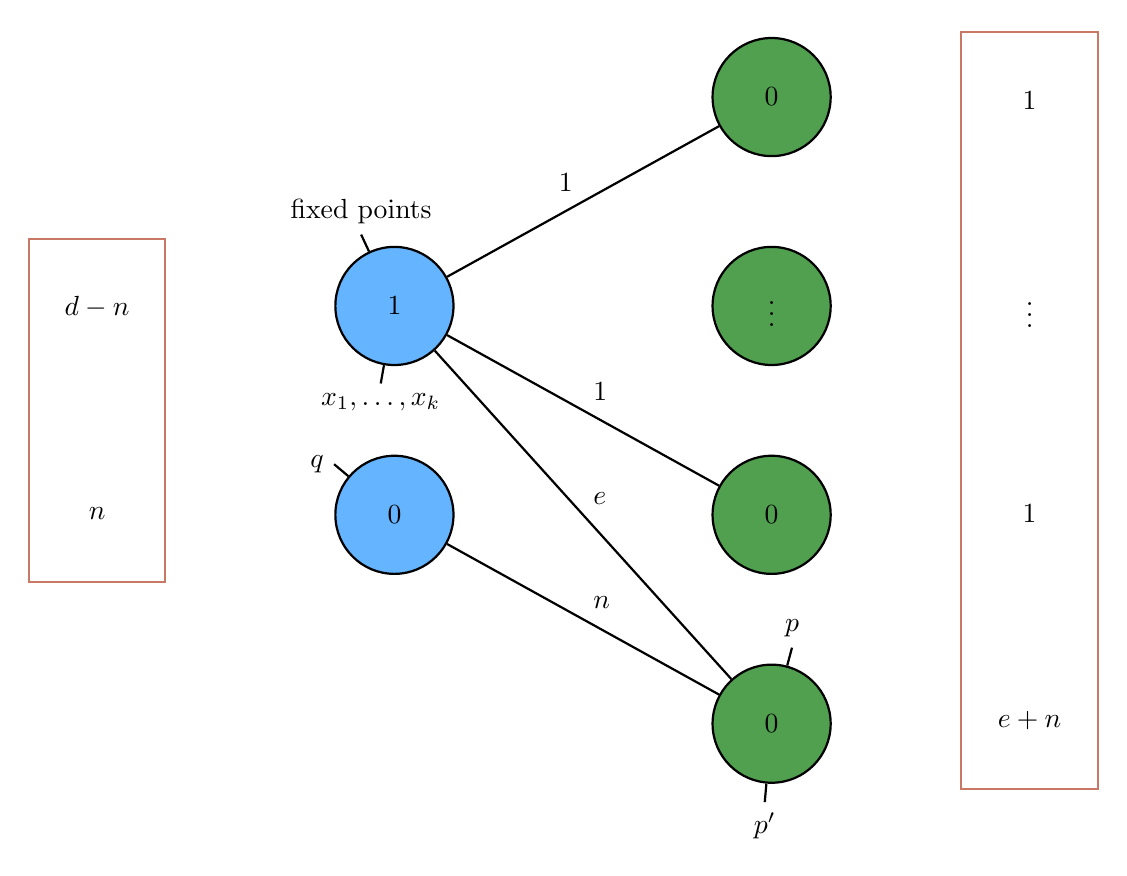
\begin{tikzpicture}[thick,amat/.style={matrix of nodes,nodes in empty cells,
  row sep=3.2em,rounded corners,
  nodes={draw,solid,circle,minimum size=1.5cm}},
  dmat/.style={matrix of nodes,nodes in empty cells,row sep=3.2em,nodes={minimum size=1.5cm},draw=myred},
  fsnode/.style={fill=myblue},
  ssnode/.style={fill=mygreen}]

  \matrix[amat,nodes=fsnode] (mat1) {$1$\\
    $0$\\};

  \matrix[dmat,left=2cm of mat1] (degrees1) {$d-n$\\
    $n$\\};

 \matrix[amat,right=3cm of mat1,nodes=ssnode] (mat2) {$0$\\
   \vdots\\
   $0$ \\
   $0$\\};
 \matrix[dmat,right=1.5cm of mat2] (degrees2) {$1$\\
   \vdots\\
   $1$ \\
   $e+n$\\};

 \draw  (mat1-1-1) edge["$1$"] (mat2-1-1)
 (mat1-1-1) edge["$1$"] (mat2-3-1)
 (mat1-1-1) edge["$e$"] (mat2-4-1)
 (mat1-2-1) edge["$n$"] (mat2-4-1);

  % draw legs for left side
 \draw (mat1-1-1) -- +(115:1) node[anchor=south] {fixed points}
 (mat1-1-1) -- +(260:1) node[anchor=north] {$x_1,\dots,x_k$}
 (mat1-2-1) -- +(140:1) node[anchor=east] {$q$};

   % draw legs for right side
 \draw (mat2-4-1) -- +(75:1) node[anchor=south] {$p$}
 (mat2-4-1) -- +(265:1) node[anchor=north] {$p'$};


        \end{tikzpicture}

        By Riemann-Hurwitz for the bottom-right component, 
        \[
        (e+n-2)+(y-1)+(z-1)=2(e+n)-2\implies y+z-2=e+n\implies e=y+z-n-2.
        \]
        By our calculation of $H((y+z-n-2,n),(z,1,\dots),(y,1,\dots))$ (and noting that
        we should multiply by $2$ if $y+z-n-2=n$, since the corresponding edges should be
        distinguished), we end up with the term in the claim.
        
\end{proof}

\subsection{Reduction of $\a$}
\begin{claim}[Claim 2]
  For $n>0$,
  \begin{align*}
    S_{\a,\b}(\mu, n, m) &= \sum_{z\in\mathfrak a,\ z\leq n+m}\min(n,m,z-1,n+m-z+1)S_{\a-\{z\},\b}(\mu,n+m-z+2) \\
    &+\sum_{z_1,z_2\in\a-\{2\}}\hat H((z_1+z_2-n-m-3,n,m),(z_1,1,\dots),(z_2,1,\dots))S_{\a-\{z_1,z_2\},\b+\{z_1+z_2-n-m-3\}}(\mu)
  \end{align*}
\end{claim}
Here $\hat H$ means  ``multiply by $|\Aut(n,m,z_1+z_2-n-m-3)|/|\Aut(z_1,z_2)|$''.

\begin{proof}
    We consider diagrams which stabilize to a genus $1$ curve containing $x_1,\dots,x_k$ and all 
  of the other fixed points, attached to a genus $0$ tail containing $q$ (with ramification index $n$) and $r$
  (with ramification index $m$).
  
  If $x_1,\dots,x_k,q,r$ are on the right side, then there is one more branch point arising as the image of some $s$ (with
  ramification index $z$). Suppose $q$ and $r$ are on different components:

  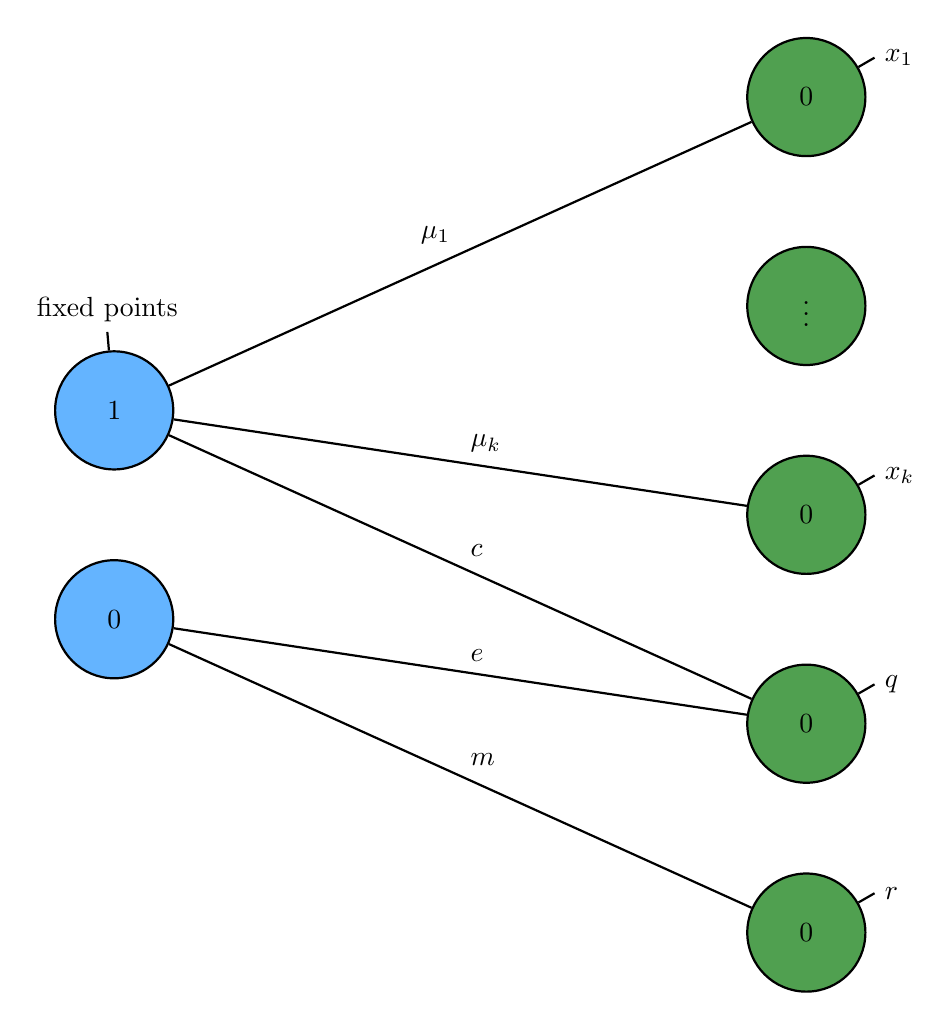
\begin{tikzpicture}[thick,amat/.style={matrix of nodes,nodes in empty cells,
  row sep=3.2em,rounded corners,
  nodes={draw,solid,circle,minimum size=1.5cm}},
  dmat/.style={matrix of nodes,nodes in empty cells,row sep=3.2em,nodes={minimum size=1.5cm},draw=myred},
  fsnode/.style={fill=myblue},
  ssnode/.style={fill=mygreen}]

  \matrix[amat,nodes=fsnode] (mat1) {$1$\\
    $0$\\};

 \matrix[amat,right=7cm of mat1,nodes=ssnode] (mat2) {$0$\\
   \vdots\\
   $0$ \\
   $0$\\
 $0$\\};

 \draw  (mat1-1-1) edge["$\mu_1$"] (mat2-1-1)
 (mat1-1-1) edge["$\mu_k$"] (mat2-3-1)
 (mat1-1-1) edge["$c$"] (mat2-4-1)
 (mat1-2-1) edge["$e$"] (mat2-4-1)
 (mat1-2-1) edge["$m$"] (mat2-5-1);

  % draw legs for left side
 \draw (mat1-1-1) -- +(95:1) node[anchor=south] {fixed points};

 % draw legs for right side
 \draw  (mat2-1-1) -- +(30:1) node[anchor=west] {$x_1$}
 (mat2-3-1) -- +(30:1) node[anchor=west] {$x_k$}
 (mat2-4-1) -- +(30:1) node[anchor=west] {$q$}
 (mat2-5-1) -- +(30:1) node[anchor=west] {$r$};

  \end{tikzpicture}

  (Without loss of generality, we suppose the component containing $q$ is the one that connects to the genus $1$.)
  There is extra ramification on both the component containing $q$ and the lower left component, a contradiction. Therefore
  $q$ and $r$ lie on the same component, and our picture must look like:

    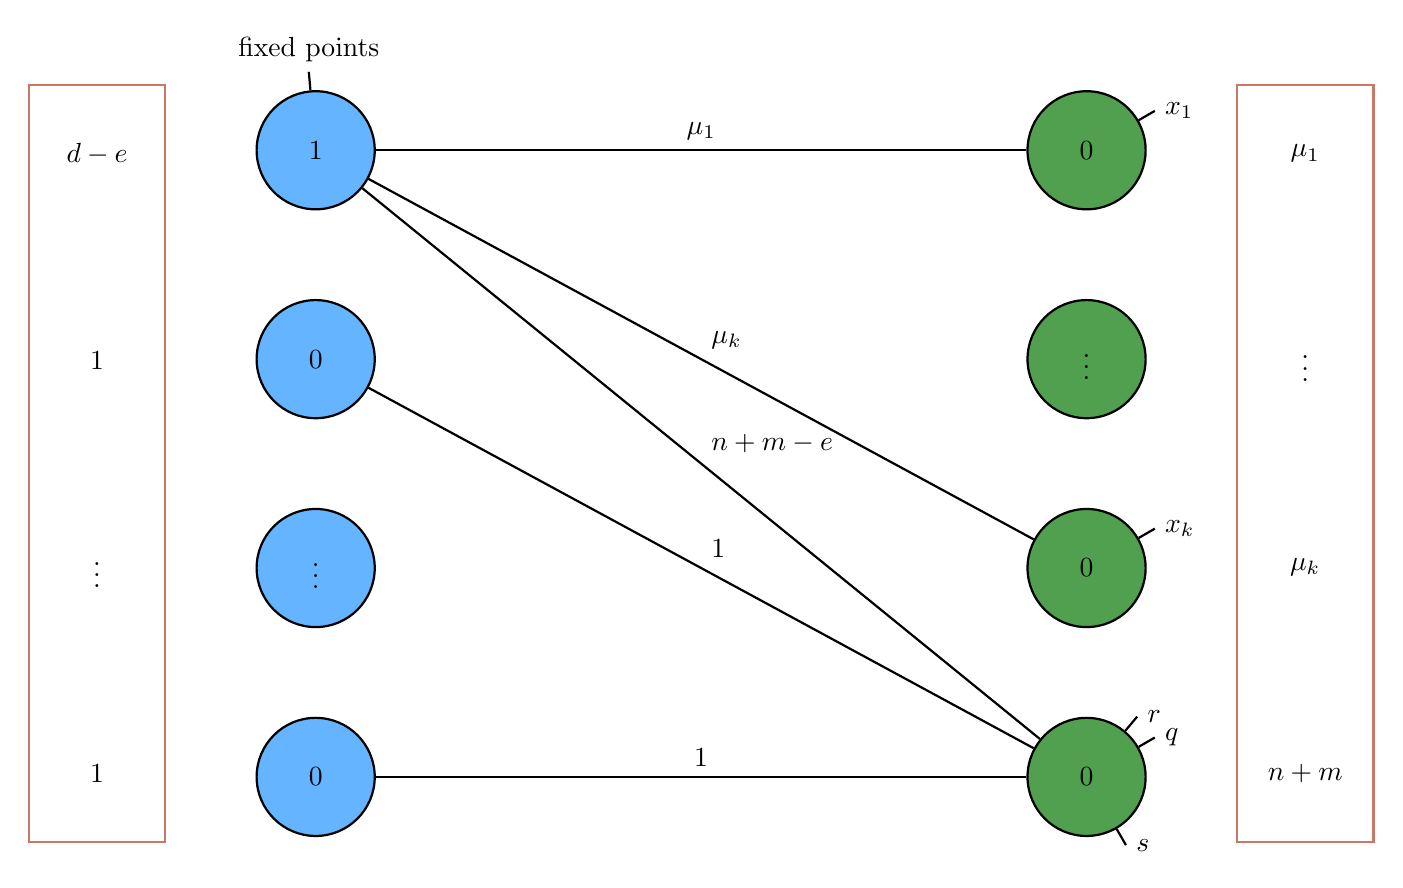
\begin{tikzpicture}[thick,amat/.style={matrix of nodes,nodes in empty cells,
  row sep=3.2em,rounded corners,
  nodes={draw,solid,circle,minimum size=1.5cm}},
  dmat/.style={matrix of nodes,nodes in empty cells,row sep=3.2em,nodes={minimum size=1.5cm},draw=myred},
  fsnode/.style={fill=myblue},
  ssnode/.style={fill=mygreen}]

  \matrix[amat,nodes=fsnode] (mat1) {$1$\\
    $0$\\
    \vdots\\
    $0$\\};

    \matrix[dmat,left=1cm of mat1] (degrees1) {$d-e$\\
    $1$\\
    \vdots \\
  $1$\\};


 \matrix[amat,right=8cm of mat1,nodes=ssnode] (mat2) {$0$\\
   \vdots\\
   $0$ \\
   $0$\\};

     \matrix[dmat,right=1cm of mat2] (degrees2) {$\mu_1$\\
    \vdots \\
    $\mu_k$\\
     $n+m$\\};

 \draw  (mat1-1-1) edge["$\mu_1$"] (mat2-1-1)
 (mat1-1-1) edge["$\mu_k$"] (mat2-3-1)
 (mat1-1-1) edge["$n+m-e$"] (mat2-4-1)
 (mat1-2-1) edge["$1$"] (mat2-4-1)
 (mat1-4-1) edge["$1$"] (mat2-4-1);

  % draw legs for left side
 \draw (mat1-1-1) -- +(95:1) node[anchor=south] {fixed points};

 % draw legs for right side
 \draw  (mat2-1-1) -- +(30:1) node[anchor=west] {$x_1$}
 (mat2-3-1) -- +(30:1) node[anchor=west] {$x_k$}
 (mat2-4-1) -- +(30:1) node[anchor=west] {$q$}
 (mat2-4-1) -- +(50:1) node[anchor=west] {$r$}
 (mat2-4-1) -- +(300:1) node[anchor=west] {$s$};

    \end{tikzpicture}

    By Riemann-Hurwitz for the lower right component,
    \[
    (n+m-e-1)+(n+m-2)+(z-1)=2(n+m)-2\implies e=z-2
    \]
    yielding the first term in the claim using our calculation of Hurwitz numbers to simplify
    $H((n,m),(z,1,\dots),(n+m-z+2,1,\dots))$.

    If $x_1,\dots,x_k,q,r$ are on the left side, then there are two branch points arising as the images of $s_1$ (with
    ramification index $z_1$) and $s_2$ (with ramification index $z_2$). By logic similar to the last proof, the
    $x_1,\dots,x_k$ all lie on the genus $1$ component.

    Consider the possibility that $q$ and $r$ lie on the same component:

      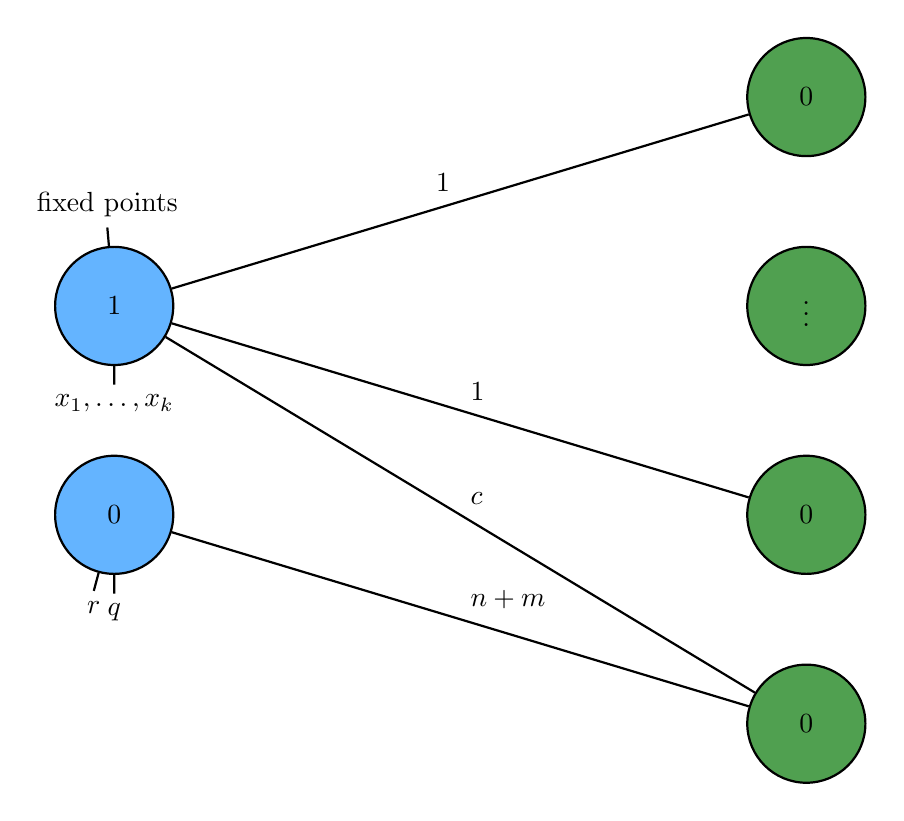
\begin{tikzpicture}[thick,amat/.style={matrix of nodes,nodes in empty cells,
  row sep=3.2em,rounded corners,
  nodes={draw,solid,circle,minimum size=1.5cm}},
  dmat/.style={matrix of nodes,nodes in empty cells,row sep=3.2em,nodes={minimum size=1.5cm},draw=myred},
  fsnode/.style={fill=myblue},
  ssnode/.style={fill=mygreen}]

  \matrix[amat,nodes=fsnode] (mat1) {$1$\\
    $0$\\};

 \matrix[amat,right=7cm of mat1,nodes=ssnode] (mat2) {$0$\\
   \vdots\\
   $0$ \\
 $0$\\};

 \draw  (mat1-1-1) edge["$1$"] (mat2-1-1)
 (mat1-1-1) edge["$1$"] (mat2-3-1)
 (mat1-1-1) edge["$c$"] (mat2-4-1)
 (mat1-2-1) edge["$n+m$"] (mat2-4-1);

  % draw legs for left side
 \draw (mat1-1-1) -- +(95:1) node[anchor=south] {fixed points}
 (mat1-1-1) -- +(270:1) node[anchor=north] {$x_1,\dots,x_k$}
 (mat1-2-1) -- +(270:1) node[anchor=north] {$q$}
 (mat1-2-1) -- +(255:1) node[anchor=north] {$r$};

      \end{tikzpicture}

      There must be at least one additional branch point from the lower left component and at least two additional branch
      points from the lower right component, a contradiction. Therefore, $q$ and $r$ lie on separate components:

          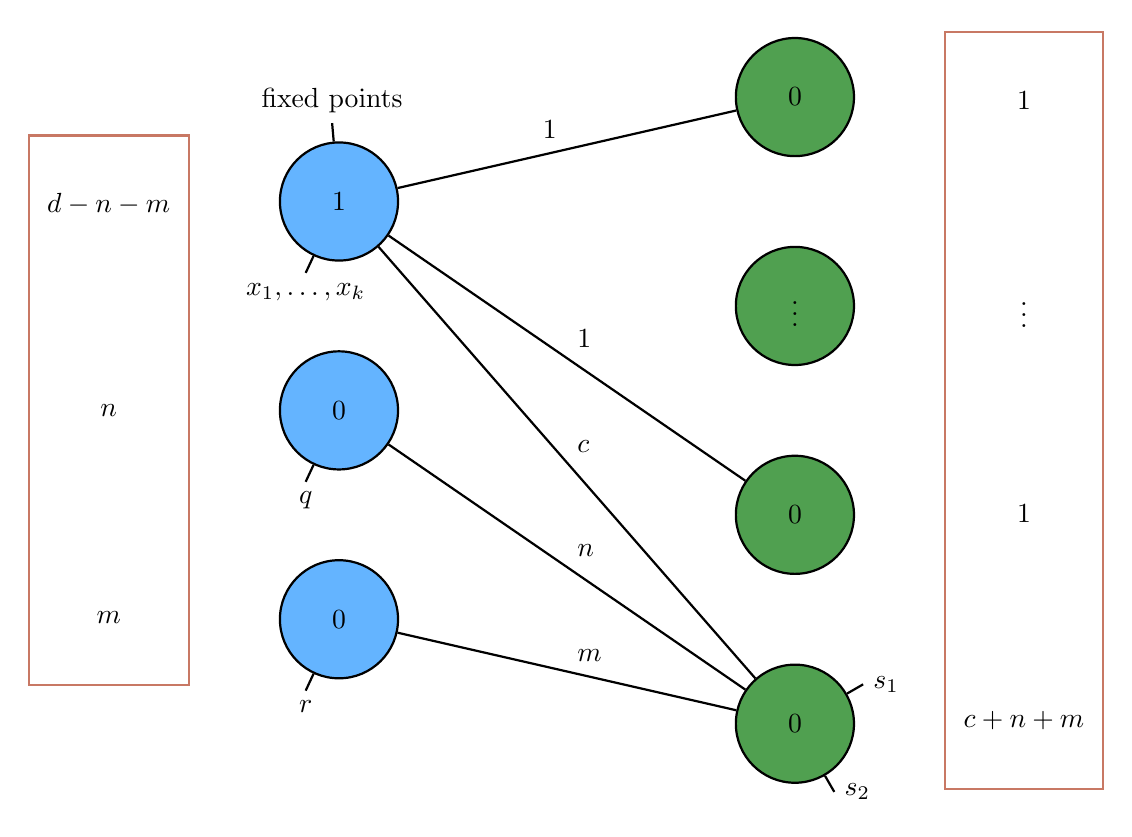
\begin{tikzpicture}[thick,amat/.style={matrix of nodes,nodes in empty cells,
  row sep=3.2em,rounded corners,
  nodes={draw,solid,circle,minimum size=1.5cm}},
  dmat/.style={matrix of nodes,nodes in empty cells,row sep=3.2em,nodes={minimum size=1.5cm},draw=myred},
  fsnode/.style={fill=myblue},
  ssnode/.style={fill=mygreen}]

  \matrix[amat,nodes=fsnode] (mat1) {$1$\\
    $0$\\
    $0$\\};

    \matrix[dmat,left=1cm of mat1] (degrees1) {$d-n-m$\\
    $n$\\
  $m$\\};


 \matrix[amat,right=4cm of mat1,nodes=ssnode] (mat2) {$0$\\
   \vdots\\
   $0$ \\
   $0$\\};

     \matrix[dmat,right=1cm of mat2] (degrees2) {$1$\\
    \vdots \\
    $1$\\
     $c+n+m$\\};

 \draw  (mat1-1-1) edge["$1$"] (mat2-1-1)
 (mat1-1-1) edge["$1$"] (mat2-3-1)
 (mat1-1-1) edge["$c$"] (mat2-4-1)
 (mat1-2-1) edge["$n$"] (mat2-4-1)
 (mat1-3-1) edge["$m$"] (mat2-4-1);

  % draw legs for left side
 \draw (mat1-1-1) -- +(95:1) node[anchor=south] {fixed points}
 (mat1-1-1) -- +(245:1) node[anchor=north] {$x_1,\dots,x_k$}
 (mat1-2-1) -- +(245:1) node[anchor=north] {$q$}
 (mat1-3-1) -- +(245:1) node[anchor=north] {$r$};

 % draw legs for right side
 \draw  (mat2-4-1) -- +(30:1) node[anchor=west] {$s_1$}
 (mat2-4-1) -- +(300:1) node[anchor=west] {$s_2$};

          \end{tikzpicture}
          
          By Riemann-Hurwitz for the lower-right component,
          \[
          (c+n+m-3)+(z_1-1)+(z_2-1)=2(c+n+m)-2\implies c=z_1+z_2-n-m-3
          \]
          yielding the second term of the claim. The additional factors arise because
          the edges from the bottom right component should be distinguished, while $s_1$ and
          $s_2$ should not be distinguished.
\end{proof}

Claim 1 allows us to reduce to the case where $\b=\emptyset$, and Claim 2 allows us to reduce to
the case where $\mu=(d)$. It remains to calculate $S_{\{a_1,a_2,a_3\},\emptyset}(d)$ as a base case:

\begin{claim}
  When $\a=\{a_1,a_2,a_3\}$, $S_{\a,\emptyset}(d)$ is given by
  \[
  \sum_{i=1}^3\sum_{e+f=d-a_i+2}\frac{2(a_j+a_k+2) H((d),(a_1,1,\dots),(e,f,1,\dots)) H((e,f),(a_j,1,\dots),(a_k,1,\dots)) |\Aut(e,f,1^{d-e-f})|}{(a_i-2)!|\Aut(a_1,a_2,a_3)|}
  \]
  where $\{1,2,3\}=\{i,j,k\}$.
\end{claim}
\begin{proof}
  We will want to calculate $W_{(d),(a_1,1,\dots),(a_2,1,\dots),(a_3,1,\dots),(2,1,\dots)^{k}}$ (where $k=d+4-a_1-a_2-a_3$ by Riemann-Hurwitz) and then divide by \[(d-a_1)!(d-a_2)!(d-a_3)!((d-1)!)^kk!|\Aut(a_1,a_2,a_3)|\]
  The pictures to consider look like:

            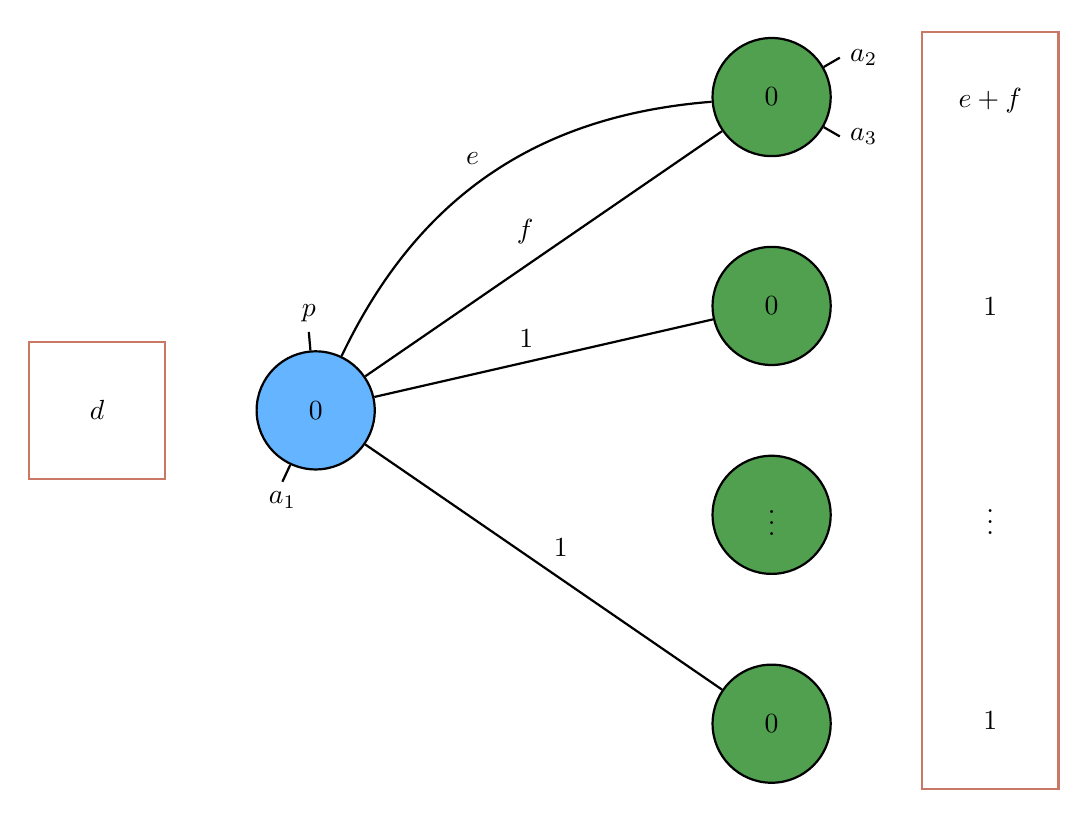
\begin{tikzpicture}[thick,amat/.style={matrix of nodes,nodes in empty cells,
  row sep=3.2em,rounded corners,
  nodes={draw,solid,circle,minimum size=1.5cm}},
  dmat/.style={matrix of nodes,nodes in empty cells,row sep=3.2em,nodes={minimum size=1.5cm},draw=myred},
  fsnode/.style={fill=myblue},
  ssnode/.style={fill=mygreen}]

  \matrix[amat,nodes=fsnode] (mat1) {$0$\\};

    \matrix[dmat,left=1cm of mat1] (degrees1) {$d$\\};


 \matrix[amat,right=4cm of mat1,nodes=ssnode] (mat2) {$0$\\
      $0$\\
      $\vdots$\\
  $0$\\};

 \matrix[dmat,right=1cm of mat2] (degrees2) {$e+f$\\
   $1$ \\
    \vdots \\
    $1$\\};

 \draw  (mat1-1-1) edge["$e$",bend left] (mat2-1-1)
 (mat1-1-1) edge["$f$"] (mat2-1-1)
 (mat1-1-1) edge["$1$"] (mat2-2-1)
 (mat1-1-1) edge["$1$"] (mat2-4-1);

  % draw legs for left side
 \draw (mat1-1-1) -- +(95:1) node[anchor=south] {$p$}
 (mat1-1-1) -- +(245:1) node[anchor=north] {$a_1$};

 % draw legs for right side
 \draw  (mat2-1-1) -- +(30:1) node[anchor=west] {$a_2$}
 (mat2-1-1) -- +(330:1) node[anchor=west] {$a_3$};

          \end{tikzpicture}

\end{proof}

\subsection{Applying recursions}

TODO: proof that Claims 1 and 2 suffice to calculate all
$S_{\a,\b}$ from base cases

We will now use the recursions to study families
\[T_n(\mu)=S_{\{n^k,2^{\ell}\},\emptyset}(\mu)\]
for fixed $n$, where $k$ is as large as possible
and then $\ell$ is determined by Riemann-Hurwitz. As a first
case, we have
\[
T_3(\mu)=S_{\{(3^{d-2}),(2^{\ell})\},\emptyset}(\mu)
\]

We find that:
\[
T_3(\mu,a,1)=T_3(\mu,a+1)+T_3(\mu,a)\text{ for $a>1$}
\]
\[
T_3(\mu,a,2)=T_3(\mu,a+2)+2T_3(\mu,a+1)\text{ for $a\geq 2$}
\]
\[
T_3(\mu,3,3)=T_3(\mu,6)+2T_3(\mu,5)
\]
and $T_3(\mu,a,b)=0$ if $a+b>6$ (for dimension reasons; TODO how does this fit with the last claim?).

\begin{claim}
  For $d\geq 3$,
  \[
  T_3(1^d)=\frac{d(d-1)(2(d-1)^2+1)}{6}
  \]
\end{claim}


TODO: Generating functions

Future questions: what does $T_n(1,\dots,1)$ look like asymptotically in $k$?

What about higher genus?

\section{Appendix 1: Hurwitz Counts}

\begin{lem}
  Let $d=2k$ be even. In the symmetric group $S_d$, if $\tau$ and $\sigma$ are products of $k$ disjoint
  transposition with $X=\sigma\tau$ consisting of two disjoint cycles, then $X$
  consists of two disjoint $k$-cycles and there exist
  $x_1,\dots,x_{k-1}$ such that
  \[
  \{1,\dots,d\}=\{1,x_1,\dots,x_{k-1},\tau(1),\tau(x_1),\dots,\tau(x_{k-1})\},
  \]
  and:
  \begin{itemize}
  \item $\sigma(1)=x_1$, 
  \item $\sigma(\tau(x_{j-2}))=x_j$ for $1<j<k$ (here $x_0=1$),
  \item $\sigma(\tau(x_{k-2}))= \tau(x_{k-1}))$.
  \end{itemize}
\end{lem}
\begin{proof}
  This can be shown by induction on $j$ (the base case, $j=1$, amounts to choosing $x_1=\sigma(1)$).
  Assume the claim up through $j-1$, i.e.\ there exist
  $x_1,\dots,x_{j-1}$ with the given properties and
  \[\{1,\dots,2j\}=\{1,x_1,\dots,x_{j-1},\tau(1),\tau(x_1),\dots,\tau(x_{j-1})\}\]

  Let $x_j$ be
  the image of $\tau(x_{j-2})$ under $\sigma$.
  We know $x_j$ is distinct from $1,x_1,\dots,x_{j-1},\tau(1),\dots,\tau(x_{j-2})$
  as these have been assigned values under $\sigma$ already (and the last is impossible
  since $\sigma$ has no fixed points).
  If $x_j=\tau(x_{j-1})$, then $X=\sigma\tau$ contains a cycle
  which looks like
  \[
  1\to x_2\to x_4\to\cdots\to x_{j-2}\to \tau(x_{j-1})\to \tau(x_{j-3})\to\cdots\to \tau(x_1)\to 1
  \]
  if $j$ is even or
  \[
  1\to x_2\to x_4\to\cdots\to x_{j-1}\to \tau(x_{j-2})\to \tau(x_{j-4})\to\cdots\to \tau(x_1)
  \]
  if $j$ is odd, both of which are length $j$. The orbit of the point $\tau(1)$ produces
  another cycle of length $j$. These two cycles involve $2j$ points.
  Under the assumption that $X$ overall consists of only
  two disjoint cycles, this is impossible if $j<k$, in which case
  \[
  \{1,x_1,\dots,x_{j},\tau(1),\dots,\tau(x_{j})\}=\{1,\dots,2j+2\}
  \]
  completing the inductive claim. On the other hand if $j=k$, then
  we are forced to have $x_k=\tau(x_{k-1})$
  and $X$ consists of two disjoint $k$-cycles.

  \end{proof}

\begin{claim}
For $d=2k$ even,
\[
H((d),(2^k),(2^k),(2,1^{d-2}))=\frac k2
\]
\end{claim}
\begin{proof}
  In the symmetric group $S_d$, let $\tau$ and $\sigma$
  be products of $k$ disjoint transpositions, with $X=\sigma\tau$ consisting
  of two disjoint cycles.

  
  The number of pairs $(\tau,\sigma)$ whose product consists of two
  disjoint cycles is the number of possibilities for $\tau$, i.e.
  \[
  (d-1)(d-3)\cdots (1),
  \]
  multiplied by the number of possibilities for $\sigma$ given $\tau$, which is
  \[
  (d-2)(d-4)\cdots (2).\]
  A permutation consisting of two disjoint cycles
  is uniquely a $d$-cycle multipled by a transposition, and
  a $d$-cycle can be written as a product of two $k$-cycles multipled by a
  transposition if the transposition interchanges a point of one $k$-cycle
  with a point of another; there are $k^2$ such transpositions.

  Thus, our Hurwitz count is
  \begin{align*}
  \frac 1{d!}\cdot ((d-1)(d-3)\cdots 1)\cdot  ((d-2)(d-4)\cdots 2)\cdot\left(\frac d2\right)^2 = \frac{1}{d}\cdot\frac{d^2}{4}=\frac k2
  \end{align*}
  as claimed.
\end{proof}

\begin{claim}
  For $d=2k$ even,
  \[
  H((2^k),(2^k),(a,b))=\begin{cases}
  \frac 1d & a=b=k \\
  0 & \text{else}
  \end{cases}
  \]
\end{claim}
\begin{proof}
  This is a result of the lemma above.
  \end{proof}

\begin{claim}
For $d=2k$ even,
\[
H((d),(2^k),(2^{k-1},1,1))=1
\]
\end{claim}

\begin{claim}
For $d=2k+1$ odd,
\[
H((d),(2^k,1),(2^{k},1))=1
\]
\end{claim}

\begin{claim}
For $2\leq a\leq d-1$,
\[
H((d),(a,1,\dots,1),(d-a+1,1,\dots,1))=1
\]
\end{claim}

\begin{claim}
  If $a+b-2=d$, $1\leq n\leq d/2$, and $2\leq a\leq d/2+1$ (equivalently $2\leq a\leq b$), then
\[
H((d-n,n),(a,1,\dots,1),(b,1,\dots,1))=\begin{cases}
\frac 12\min(a-1,n)& d=2n \\
\min(a-1,n)&\text{else}
\end{cases}
\]
\end{claim}
\begin{proof}
  We want to count choices of an $a$-cycle and a $b$-cycle which compose to produce cycle type $(d-n,n)$.
  There are $\binom da$ choices for the points of the $a$-cycle, and the
  points of the $b$-cycle are determined by the two points $x$,$y$ the cycles have in common, of which there are $\binom a2$
  choices.
  Composing these cycles yields cycle type $(n,d-n)$ where $n=n_1+n_2-1$ and
  \[
  n_1=\text{dist}_a(y,x),\quad n_2=\text{dist}_b(x,y)
  \]
  since $y$ can be traced for $n_1-1$ steps along the $a$-cycle to the predecessor of $x$, which then leads to
  the successor of $y$ in the $b$-cycle and another $n_2-1$ steps to reach $x$ again.

  If $n_1$ is fixed, there are $\frac{(a-1)!}{a-1}$ orientations of the $a$-cycle with given $\text{dist}_a(y,x)$ and similarly for the $b$-cycle,
  so our count is
  \[
  \binom da\cdot \binom a2\cdot \frac{(a-1)!}{a-1}\cdot\frac{(b-1)!}{b-1}\sum_{n_1+n_2=n+1}1
  \]
  This yields $\frac 12d!\cdot\min(a-1,n)$, and if $d\neq 2n$ then we multiply by $2$ to account for the case where $n_1+n_2-1=d-n$ instead of $n$.
  \end{proof}

\begin{claim}
  If $a+b-3=d$, $n+m+p=d$, $1\leq n\leq m\leq p$, and $3\leq a\leq \frac{d+3}{2}$ (equivalently $2\leq a\leq b$), then
\begin{align*}
  H((n,m,p),&(a,1,\dots,1),(b,1,\dots,1))\\
  &=\frac 2{|\Aut(n,m,p)|}\cdot \#\{(n_1,m_1):1\leq n_1\leq n,\ \max(1,a-p-n_1)\leq m_1\leq \min(m,a-1-n_1)\}
\end{align*}
In particular if $n=m=1$ and $d>3$, the Hurwitz number is $1$.
\end{claim}
\begin{proof}
  We want to count choices of an $a$-cycle and a $b$-cycle which compose to produce cycle type $(n,m,p)$.
  There are $\binom da$ choices for the points of the $a$-cycle, and the
  points of the $b$-cycle will be determined by the three points $x,y,z$ the cycles have in common. We have $a$ choices for
  $x$ (we will need to divide by $3$ later to account for the fact that $x,y,z$ are unordered).

  If the directionality of the $a$-cycle is $x\to y\to z\to x$ (WLOG), then the same directionality in the $b$-cycle would lead to
  a $d$-cycle, so we will require $x\to z\to y\to x$ in the $b$-cycle to end up with the desired cycle type. In this case
  we have a composed chain \[x\to\cdots\to \text{pred}_a(y)\to\text{succ}_b(y)\cdots\to x\] of length $n_1+n_2-1$ where $n_1=\text{dist}_a(x,y)$ and $n_2=\text{dist}_b(y,x)$, and similarly a composed chain
  \[
  y\to\cdots\to\text{pred}_a(z)\to\text{succ}_b(z)\to\cdots\to y
  \]
  of length $m_1+m_2-1$ where $m_1=\text{dist}_a(y,z)$ and $m_2=\text{dist}_b(z,y)$.

  Choose $n_1,n_2,m_1,m_2$ such that $n_1+n_2-1=n$ and $m_1+m_2-1=m$. Then there are $(a-1)!$ orientations of the $a$-cycle, and $y$ and $z$ are determined by $n_1$ and $m_1$. There are then $(b-3)!$ orientations of the $b$-cycle respecting the gaps $n_2$ and $m_2$. Finally, the number of choices we have in choosing $n,m$ this way out of $n,m,p$ is $\frac{3!}{|\Aut(n,m,p)|}$, so
  \begin{align*}
    H((n,m,p),(a,1,\dots,1),(b,1,\dots,1))&=\binom da\cdot a\cdot\frac 13\cdot\sum_{n_1,n_2,m_1,m_2}(a-1)!(b-3)!\cdot\frac{3!}{|\Aut(n,m,p)|} \\
    &=\frac{d!}{a!(d-a)!}\cdot\frac a3\cdot\frac{(a-1)!(d-a)!\cdot 6}{|\Aut(n,m,p)|}\#\{n_1,n_2,m_1,m_2\}
  \end{align*}
  yielding the result.
  
\end{proof}

\begin{claim}
  If $1\leq a\leq d$, $2\leq b\leq d-2$, $2\leq c\leq d-2$, and $a+b+c=d+2$, then
  \[
  H((d),(a,1,\dots),(b,c,1,\dots))=\frac{a-1}{|\Aut(b,c)|}.
  \]
  (By the first claim of this document, the Hurwitz number is $1$ if $b=1$ or $c=1$ but not both, and it is $1/d$ if $b=c=1$.)
\end{claim}
\begin{proof}
  We want to multiply an $a$-cycle by a disjoint $b$-cycle and $c$-cycle to get a $d$-cycle; the only
  requirement is that the $a$-cycle has a point $x$ contained in the $b$-cycle and a point $y$ contained in the
  $c$-cycle.
  The count is
  \[
  \binom da\cdot (a-1)!\cdot (a(a-1))\cdot \binom{d-a}{b-1}\cdot (b-1)!\cdot (c-1)!\cdot \frac 1{|\Aut(b,c)|}
  \]
  which comes out to
  \[
  d!\cdot\frac{a-1}{|\Aut(b,c)|}.
  \]
  \end{proof}

\printbibliography

\end{document}
